\documentclass[preprint]{sigplanconf}

\usepackage{amssymb}
\usepackage{amsthm}
\usepackage{breakurl}             % Not needed if you use pdflatex only.
\usepackage{color}
\usepackage{epsfig}
\usepackage{esvect}
\usepackage{listings}
\usepackage{mathpartir}
\usepackage{MnSymbol}
\usepackage{multirow}
\usepackage{rotating}

\lstdefinestyle{Caml}{language=Caml,%
  literate={when}{{{\bf when}}}4
}

\lstdefinestyle{C++}{language=C++,%
showstringspaces=false,
  columns=fullflexible,
  escapechar=@,
  basicstyle=\sffamily,
%  commentstyle=\rmfamily\itshape,
  moredelim=**[is][\color{white}]{~}{~},
  literate={[<]}{{\textless}}1      {[>]}{{\textgreater}}1 %
           {<}{{$\langle$}}1        {>}{{$\rangle$}}1 %
           {<=}{{$\leq$}}1          {>=}{{$\geq$}}1          
           {==}{{$==$}}2            {!=}{{$\neq$}}1 %
           {=>}{{$\Rightarrow\;$}}1 {->}{{$\rightarrow{}$}}1 %
           {<:}{{$\subtype{}\ $}}1  {<-}{{$\leftarrow$}}1 %
           {e1}{{$e_1$}}2 {e2}{{$e_2$}}2 {e3}{{$e_3$}}2 {e4}{{$e_4$}}2%
           {E1}{{$E_1$}}2 {E2}{{$E_2$}}2 {E3}{{$E_3$}}2 {E4}{{$E_4$}}2%
           {m_e1}{{$m\_e_1$}}4 {m_e2}{{$m\_e_2$}}4 {m_e3}{{$m\_e_3$}}4 {m_e4}{{$m\_e_4$}}4%
           {Match}{{\emph{Match}}}5 %
           {Case}{{\emph{Case}}}4 %
           {Que}{{\emph{Que}}}3 %
           {Otherwise}{{\emph{Otherwise}}}9 %
           {EndMatch}{{\emph{EndMatch}}}8 %
           {CM}{{\emph{CM}}}2 {KS}{{\emph{KS}}}2 {KV}{{\emph{KV}}}2 
}
\lstset{style=C++}
\DeclareRobustCommand{\code}[1]{{\lstinline[breaklines=false,escapechar=@]{#1}}}
\DeclareRobustCommand{\codehaskell}[1]{{\lstinline[breaklines=false,language=Haskell]{#1}}}
\DeclareRobustCommand{\codeocaml}[1]{{\lstinline[breaklines=false,language=Caml]{#1}}}

\newtheorem{theorem}{Theorem}
\newtheorem{corollary}{Corollary}

%% grammar commands
\newcommand{\Rule}[1]{{\rmfamily\itshape{#1}}}
\newcommand{\Alt}{\ensuremath{|}}
\newcommand{\is}{$::=$}
\newcommand{\subtype}{\textless:}
\newcommand{\evals}{\Rightarrow}
\newcommand{\evalspp}{\Rightarrow^+}
\newcommand{\DynCast}[2]{\ensuremath{dc\langle{#1}\rangle({#2})}}
\newcommand{\nullptr}{\ensuremath{\bot}}

\newcommand{\f}[1]{{ {\bf \textcolor{blue}{#1\%}}}}
\newcommand{\s}[1]{{ {\em \textcolor{cyan}{#1\%}}}}
\newcommand{\n}[1]{{ {\bf ~ ~ ~ ~ }}}
\newcommand{\Opn}{{\scriptsize {\bf Open}}}
\newcommand{\Cls}{{\scriptsize {\bf Tag}}}
\newcommand{\Unn}{{\scriptsize {\bf Union}}}

%\newcommand{\gwNGPp}{\n{}}
%\newcommand{\gwNGKp}{\n{}}
 \newcommand{\gwNGUp}{\n{}}
%\newcommand{\gwNSPp}{\n{}}
%\newcommand{\gwNSKp}{\n{}}
 \newcommand{\gwNSUp}{\n{}}
%\newcommand{\vwNGPp}{\n{}}
%\newcommand{\vwNGKp}{\n{}}
 \newcommand{\vwNGUp}{\n{}}
%\newcommand{\vwNSPp}{\n{}}
%\newcommand{\vwNSKp}{\n{}}
 \newcommand{\vwNSUp}{\n{}}
%\newcommand{\vxNGPp}{\n{}}
%\newcommand{\vxNGKp}{\n{}}
 \newcommand{\vxNGUp}{\n{}}
%\newcommand{\vxNSPp}{\n{}}
%\newcommand{\vxNSKp}{\n{}}
 \newcommand{\vxNSUp}{\n{}}

%\newcommand{\gwNGPq}{\n{}}
%\newcommand{\gwNGKq}{\n{}}
 \newcommand{\gwNGUq}{\n{}}
%\newcommand{\gwNSPq}{\n{}}
%\newcommand{\gwNSKq}{\n{}}
 \newcommand{\gwNSUq}{\n{}}
%\newcommand{\vwNGPq}{\n{}}
%\newcommand{\vwNGKq}{\n{}}
 \newcommand{\vwNGUq}{\n{}}
%\newcommand{\vwNSPq}{\n{}}
%\newcommand{\vwNSKq}{\n{}}
 \newcommand{\vwNSUq}{\n{}}
%\newcommand{\vxNGPq}{\n{}}
%\newcommand{\vxNGKq}{\n{}}
 \newcommand{\vxNGUq}{\n{}}
%\newcommand{\vxNSPq}{\n{}}
%\newcommand{\vxNSKq}{\n{}}
 \newcommand{\vxNSUq}{\n{}}

%\newcommand{\gwNGPn}{\n{}}
%\newcommand{\gwNGKn}{\n{}}
 \newcommand{\gwNGUn}{\n{}}
%\newcommand{\gwNSPn}{\n{}}
%\newcommand{\gwNSKn}{\n{}}
 \newcommand{\gwNSUn}{\n{}}
%\newcommand{\vwNGPn}{\n{}}
%\newcommand{\vwNGKn}{\n{}}
 \newcommand{\vwNGUn}{\n{}}
%\newcommand{\vwNSPn}{\n{}}
%\newcommand{\vwNSKn}{\n{}}
 \newcommand{\vwNSUn}{\n{}}
%\newcommand{\vxNGPn}{\n{}}
%\newcommand{\vxNGKn}{\n{}}
 \newcommand{\vxNGUn}{\n{}}
%\newcommand{\vxNSPn}{\n{}}
%\newcommand{\vxNSKn}{\n{}}
 \newcommand{\vxNSUn}{\n{}}


%\newcommand{\gwYGPp}{\n{}}
% \newcommand{\gwYGKp}{\n{}}
 \newcommand{\gwYGUp}{\n{}}
%\newcommand{\gwYSPp}{\n{}}
% \newcommand{\gwYSKp}{\n{}}
 \newcommand{\gwYSUp}{\n{}}
%\newcommand{\vwYGPp}{\n{}}
% \newcommand{\vwYGKp}{\n{}}
 \newcommand{\vwYGUp}{\n{}}
%\newcommand{\vwYSPp}{\n{}}
% \newcommand{\vwYSKp}{\n{}}
 \newcommand{\vwYSUp}{\n{}}
%\newcommand{\vxYGPp}{\n{}}
% \newcommand{\vxYGKp}{\n{}}
 \newcommand{\vxYGUp}{\n{}}
%\newcommand{\vxYSPp}{\n{}}
% \newcommand{\vxYSKp}{\n{}}
 \newcommand{\vxYSUp}{\n{}}

%\newcommand{\gwYGPq}{\n{}}
% \newcommand{\gwYGKq}{\n{}}
 \newcommand{\gwYGUq}{\n{}}
%\newcommand{\gwYSPq}{\n{}}
% \newcommand{\gwYSKq}{\n{}}
 \newcommand{\gwYSUq}{\n{}}
%\newcommand{\vwYGPq}{\n{}}
% \newcommand{\vwYGKq}{\n{}}
 \newcommand{\vwYGUq}{\n{}}
%\newcommand{\vwYSPq}{\n{}}
% \newcommand{\vwYSKq}{\n{}}
 \newcommand{\vwYSUq}{\n{}}
%\newcommand{\vxYGPq}{\n{}}
% \newcommand{\vxYGKq}{\n{}}
 \newcommand{\vxYGUq}{\n{}}
%\newcommand{\vxYSPq}{\n{}}
% \newcommand{\vxYSKq}{\n{}}
 \newcommand{\vxYSUq}{\n{}}

%\newcommand{\gwYGPn}{\n{}}
% \newcommand{\gwYGKn}{\n{}}
 \newcommand{\gwYGUn}{\n{}}
%\newcommand{\gwYSPn}{\n{}}
% \newcommand{\gwYSKn}{\n{}}
 \newcommand{\gwYSUn}{\n{}}
%\newcommand{\vwYGPn}{\n{}}
% \newcommand{\vwYGKn}{\n{}}
 \newcommand{\vwYGUn}{\n{}}
%\newcommand{\vwYSPn}{\n{}}
% \newcommand{\vwYSKn}{\n{}}
 \newcommand{\vwYSUn}{\n{}}
%\newcommand{\vxYGPn}{\n{}}
% \newcommand{\vxYGKn}{\n{}}
 \newcommand{\vxYGUn}{\n{}}
%\newcommand{\vxYSPn}{\n{}}
% \newcommand{\vxYSKn}{\n{}}
 \newcommand{\vxYSUn}{\n{}}

 \newcommand{\GwNGPp}{\n{}}
 \newcommand{\GwNGKp}{\n{}}
 \newcommand{\GwNGUp}{\n{}}
 \newcommand{\GwNSPp}{\n{}}
 \newcommand{\GwNSKp}{\n{}}
 \newcommand{\GwNSUp}{\n{}}
%\newcommand{\VwNGPp}{\n{}}
%\newcommand{\VwNGKp}{\n{}}
 \newcommand{\VwNGUp}{\n{}}
%\newcommand{\VwNSPp}{\n{}}
%\newcommand{\VwNSKp}{\n{}}
 \newcommand{\VwNSUp}{\n{}}
%\newcommand{\VxNGPp}{\n{}}
%\newcommand{\VxNGKp}{\n{}}
 \newcommand{\VxNGUp}{\n{}}
%\newcommand{\VxNSPp}{\n{}}
%\newcommand{\VxNSKp}{\n{}}
 \newcommand{\VxNSUp}{\n{}}

 \newcommand{\GwNGPq}{\n{}}
 \newcommand{\GwNGKq}{\n{}}
 \newcommand{\GwNGUq}{\n{}}
 \newcommand{\GwNSPq}{\n{}}
 \newcommand{\GwNSKq}{\n{}}
 \newcommand{\GwNSUq}{\n{}}
%\newcommand{\VwNGPq}{\n{}}
%\newcommand{\VwNGKq}{\n{}}
 \newcommand{\VwNGUq}{\n{}}
%\newcommand{\VwNSPq}{\n{}}
%\newcommand{\VwNSKq}{\n{}}
 \newcommand{\VwNSUq}{\n{}}
%\newcommand{\VxNGPq}{\n{}}
%\newcommand{\VxNGKq}{\n{}}
 \newcommand{\VxNGUq}{\n{}}
%\newcommand{\VxNSPq}{\n{}}
%\newcommand{\VxNSKq}{\n{}}
 \newcommand{\VxNSUq}{\n{}}

 \newcommand{\GwNGPn}{\n{}}
 \newcommand{\GwNGKn}{\n{}}
 \newcommand{\GwNGUn}{\n{}}
 \newcommand{\GwNSPn}{\n{}}
 \newcommand{\GwNSKn}{\n{}}
 \newcommand{\GwNSUn}{\n{}}
%\newcommand{\VwNGPn}{\n{}}
%\newcommand{\VwNGKn}{\n{}}
 \newcommand{\VwNGUn}{\n{}}
%\newcommand{\VwNSPn}{\n{}}
%\newcommand{\VwNSKn}{\n{}}
 \newcommand{\VwNSUn}{\n{}}
%\newcommand{\VxNGPn}{\n{}}
%\newcommand{\VxNGKn}{\n{}}
 \newcommand{\VxNGUn}{\n{}}
%\newcommand{\VxNSPn}{\n{}}
%\newcommand{\VxNSKn}{\n{}}
 \newcommand{\VxNSUn}{\n{}}


 \newcommand{\GwYGPp}{\n{}}
 \newcommand{\GwYGKp}{\n{}}
 \newcommand{\GwYGUp}{\n{}}
 \newcommand{\GwYSPp}{\n{}}
 \newcommand{\GwYSKp}{\n{}}
 \newcommand{\GwYSUp}{\n{}}
%\newcommand{\VwYGPp}{\n{}}
% \newcommand{\VwYGKp}{\n{}}
 \newcommand{\VwYGUp}{\n{}}
%\newcommand{\VwYSPp}{\n{}}
% \newcommand{\VwYSKp}{\n{}}
 \newcommand{\VwYSUp}{\n{}}
%\newcommand{\VxYGPp}{\n{}}
% \newcommand{\VxYGKp}{\n{}}
 \newcommand{\VxYGUp}{\n{}}
%\newcommand{\VxYSPp}{\n{}}
% \newcommand{\VxYSKp}{\n{}}
 \newcommand{\VxYSUp}{\n{}}

 \newcommand{\GwYGPq}{\n{}}
 \newcommand{\GwYGKq}{\n{}}
 \newcommand{\GwYGUq}{\n{}}
 \newcommand{\GwYSPq}{\n{}}
 \newcommand{\GwYSKq}{\n{}}
 \newcommand{\GwYSUq}{\n{}}
%\newcommand{\VwYGPq}{\n{}}
% \newcommand{\VwYGKq}{\n{}}
 \newcommand{\VwYGUq}{\n{}}
%\newcommand{\VwYSPq}{\n{}}
% \newcommand{\VwYSKq}{\n{}}
 \newcommand{\VwYSUq}{\n{}}
%\newcommand{\VxYGPq}{\n{}}
% \newcommand{\VxYGKq}{\n{}}
 \newcommand{\VxYGUq}{\n{}}
%\newcommand{\VxYSPq}{\n{}}
% \newcommand{\VxYSKq}{\n{}}
 \newcommand{\VxYSUq}{\n{}}

 \newcommand{\GwYGPn}{\n{}}
 \newcommand{\GwYGKn}{\n{}}
 \newcommand{\GwYGUn}{\n{}}
 \newcommand{\GwYSPn}{\n{}}
 \newcommand{\GwYSKn}{\n{}}
 \newcommand{\GwYSUn}{\n{}}
%\newcommand{\VwYGPn}{\n{}}
% \newcommand{\VwYGKn}{\n{}}
 \newcommand{\VwYGUn}{\n{}}
%\newcommand{\VwYSPn}{\n{}}
% \newcommand{\VwYSKn}{\n{}}
 \newcommand{\VwYSUn}{\n{}}
%\newcommand{\VxYGPn}{\n{}}
% \newcommand{\VxYGKn}{\n{}}
 \newcommand{\VxYGUn}{\n{}}
%\newcommand{\VxYSPn}{\n{}}
% \newcommand{\VxYSKn}{\n{}}
 \newcommand{\VxYSUn}{\n{}}

% This file defines variables with performance numbers for the table in Evaluation section
% Data from 2011-08-30 
\newcommand{\vwYGKp}{\s{3}}
\newcommand{\vwYGKn}{\s{8}}
\newcommand{\vwYGKq}{\s{11}}
\newcommand{\vwYGPp}{\f{10}}
\newcommand{\vwYGPn}{\f{14}}
\newcommand{\vwYGPq}{\s{0}}
\newcommand{\vwYSKp}{\s{7}}
\newcommand{\vwYSKn}{\s{7}}
\newcommand{\vwYSKq}{\s{10}}
\newcommand{\vwYSPp}{\f{10}}
\newcommand{\vwYSPn}{\f{14}}
\newcommand{\vwYSPq}{\s{0}}
\newcommand{\vwNGKp}{\f{35}}
\newcommand{\vwNGKn}{\s{6}}
\newcommand{\vwNGKq}{\s{5}}
\newcommand{\vwNGPp}{\f{1}}
\newcommand{\vwNGPn}{\s{1}}
\newcommand{\vwNGPq}{\s{10}}
\newcommand{\vwNSKp}{\f{133}}
\newcommand{\vwNSKn}{\f{25}}
\newcommand{\vwNSKq}{\f{59}}
\newcommand{\vwNSPp}{\f{1}}
\newcommand{\vwNSPn}{\s{1}}
\newcommand{\vwNSPq}{\s{8}}

\newcommand{\vxYGKp}{\s{61}}
\newcommand{\vxYGKn}{\s{24}}
\newcommand{\vxYGKq}{\s{25}}
\newcommand{\vxYGPp}{\s{24}}
\newcommand{\vxYGPn}{\s{24}}
\newcommand{\vxYGPq}{\s{36}}
\newcommand{\vxYSKp}{\s{79}}
\newcommand{\vxYSKn}{\s{25}}
\newcommand{\vxYSKq}{\s{35}}
\newcommand{\vxYSPp}{\s{9}}
\newcommand{\vxYSPn}{\s{23}}
\newcommand{\vxYSPq}{\f{133}}
\newcommand{\vxNGKp}{\s{8}}
\newcommand{\vxNGKn}{\s{5}}
\newcommand{\vxNGKq}{\s{0}}
\newcommand{\vxNGPp}{\s{33}}
\newcommand{\vxNGPn}{\s{47}}
\newcommand{\vxNGPq}{\s{43}}
\newcommand{\vxNSKp}{\f{38}}
\newcommand{\vxNSKn}{\f{12}}
\newcommand{\vxNSKq}{\f{3}}
\newcommand{\vxNSPp}{\s{27}}
\newcommand{\vxNSPn}{\s{44}}
\newcommand{\vxNSPq}{\s{45}}

\newcommand{\gwYGKp}{\f{88}}
\newcommand{\gwYGKn}{\f{32}}
\newcommand{\gwYGKq}{\f{250}}
\newcommand{\gwYGPp}{\f{67}}
\newcommand{\gwYGPn}{\f{28}}
\newcommand{\gwYGPq}{\f{87}}
\newcommand{\gwYSKp}{\f{79}}
\newcommand{\gwYSKn}{\f{31}}
\newcommand{\gwYSKq}{\f{259}}
\newcommand{\gwYSPp}{\f{67}}
\newcommand{\gwYSPn}{\f{27}}
\newcommand{\gwYSPq}{\f{90}}
\newcommand{\gwNGKp}{\f{116}}
\newcommand{\gwNGKn}{\f{29}}
\newcommand{\gwNGKq}{\f{43}}
\newcommand{\gwNGPp}{\f{55}}
\newcommand{\gwNGPn}{\s{0}}
\newcommand{\gwNGPq}{\f{1}}
\newcommand{\gwNSKp}{\f{216}}
\newcommand{\gwNSKn}{\f{542}}
\newcommand{\gwNSKq}{\f{520}}
\newcommand{\gwNSPp}{\f{55}}
\newcommand{\gwNSPn}{\f{1}}
\newcommand{\gwNSPq}{\f{3}}

\newcommand{\VwYGKp}{\f{16}}
\newcommand{\VwYGKn}{\f{11}}
\newcommand{\VwYGKq}{\f{168}}
\newcommand{\VwYGPp}{\f{10}}
\newcommand{\VwYGPn}{\f{19}}
\newcommand{\VwYGPq}{\f{153}}
\newcommand{\VwYSKp}{\f{31}}
\newcommand{\VwYSKn}{\f{24}}
\newcommand{\VwYSKq}{\f{185}}
\newcommand{\VwYSPp}{\f{10}}
\newcommand{\VwYSPn}{\f{18}}
\newcommand{\VwYSPq}{\f{153}}
\newcommand{\VwNGKp}{\f{61}}
\newcommand{\VwNGKn}{\f{18}}
\newcommand{\VwNGKq}{\f{13}}
\newcommand{\VwNGPp}{\f{4}}
\newcommand{\VwNGPn}{\s{17}}
\newcommand{\VwNGPq}{\s{9}}
\newcommand{\VwNSKp}{\f{124}}
\newcommand{\VwNSKn}{\f{43}}
\newcommand{\VwNSKq}{\f{34}}
\newcommand{\VwNSPp}{\f{4}}
\newcommand{\VwNSPn}{\s{18}}
\newcommand{\VwNSPq}{\f{3}}
               
\newcommand{\VxYGKp}{\s{5}}
\newcommand{\VxYGKn}{\s{2}}
\newcommand{\VxYGKq}{\f{132}}
\newcommand{\VxYGPp}{\s{5}}
\newcommand{\VxYGPn}{\s{5}}
\newcommand{\VxYGPq}{\f{130}}
\newcommand{\VxYSKp}{\s{9}}
\newcommand{\VxYSKn}{\s{10}}
\newcommand{\VxYSKq}{\f{118}}
\newcommand{\VxYSPp}{\s{6}}
\newcommand{\VxYSPn}{\s{6}}
\newcommand{\VxYSPq}{\f{145}}
\newcommand{\VxNGKp}{\f{20}}
\newcommand{\VxNGKn}{\f{7}}
\newcommand{\VxNGKq}{\f{34}}
\newcommand{\VxNGPp}{\s{14}}
\newcommand{\VxNGPn}{\s{27}}
\newcommand{\VxNGPq}{\f{2}}
\newcommand{\VxNSKp}{\f{47}}
\newcommand{\VxNSKn}{\f{16}}
\newcommand{\VxNSKq}{\f{14}}
\newcommand{\VxNSPp}{\s{0}}
\newcommand{\VxNSPn}{\s{27}}
\newcommand{\VxNSPq}{\f{1}}


\newsavebox{\sembox}
\newlength{\semwidth}
\newlength{\boxwidth}

\newcommand{\Sem}[1]{%
\sbox{\sembox}{\ensuremath{#1}}%
\settowidth{\semwidth}{\usebox{\sembox}}%
\sbox{\sembox}{\ensuremath{\left[\usebox{\sembox}\right]}}%
\settowidth{\boxwidth}{\usebox{\sembox}}%
\addtolength{\boxwidth}{-\semwidth}%
\left[\hspace{-0.3\boxwidth}%
\usebox{\sembox}%
\hspace{-0.3\boxwidth}\right]%
}

\newcommand{\authormodification}[2]{{\color{#1}#2}}
\newcommand{\ys}[1]{\authormodification{blue}{#1}}
\newcommand{\bs}[1]{\authormodification{red}{#1}}
\newcommand{\gdr}[1]{\authormodification{magenta}{#1}}

\begin{document}

%\conferenceinfo{PLDI 2012}{Beijing, China} 
%\copyrightyear{2012} 
%\copyrightdata{[to be supplied]} 

\titlebanner{Draft}        % These are ignored unless
\preprintfooter{Y.Solodkyy, G.Dos Reis, B.Stroustrup: Efficient Type Switching with Memoization Device}   % 'preprint' option specified.

\title{Efficient Type Switching with Memoization Device}
%\subtitle{your \code{visit}, Jim, is not \code{accept}able anymore}
%\subtitle{\code{accepting} aint no \code{visit}ors}

\authorinfo{Yuriy Solodkyy\and Gabriel Dos Reis\and Bjarne Stroustrup}
           {Texas A\&M University\\ Texas, USA}
           {\{yuriys,gdr,bs\}@cse.tamu.edu}

\maketitle

\begin{abstract}
We present several techniques that can be used in a compiler and/or library 
setting to implement efficiently type switching, type testing, pattern matching, 
predicate dispatch, multi-methods and other facilities that depend on run-time 
type of the argument. The techniques cope well with multiple inheritance typical 
for C++, however they are not specific to C++ and can be adopted to implementation 
of similar facilities in other languages.

Our library-only implementation of a type switch based on these techniques, equals 
or outperforms visitor design pattern, as commonly used for type-casing 
scenarios in C++, and for many use cases it equals or outperforms equivalent 
code in languages with built-in type switching constructs. While remaining a 
library-only solution, such a facility better addresses expression problem 
than the visitor design pattern does: it is non-intrusive and does not have 
extensibility restrictions. It also avoids control inversion characteristic to 
visitors, making the code significantly more concise and easier to comprehend.
 
The library was motivated by and is used for applications involving large, 
typed, abstract syntax trees.
\end{abstract}

\category{CR-number}{subcategory}{third-level}

\terms
Languages, Design

\keywords
Pattern Matching, Visitor Design Pattern, Expression Problem, C++

\section{Introduction} %%%%%%%%%%%%%%%%%%%%%%%%%%%%%%%%%%%%%%%%%%%%%%%%%%%%%%%%%
\label{sec:intro}

%Motivate the problem
%Give a summary of the paper: what you did and how
%Explicitly state your contribution

%Expression problem is a problem of supporting in a programming language modular 
%extensibility of both data and functions at the same time. Functional languages
%allow for easy addition of new functions at the expense of disallowing new data
%variants. Object-oriented languages allow for easy addition of new variants at 
%the expense of disallowing new functions. Many attempts have been made to 
%resolve this dilema in both camps, nevertheless no universally accepted solution 
%that is modular, open and efficient has been found.

%Visitor Design Pattern has became de-facto standard in dealing with expression 
%problem in many industry-strength object-oriented languages because of two 
%factors: its speed and being a library solution. It comes at the cost of 
%restricting extensibility of data, increased verbosity and being hard to teach 
%and understand, but nevertheless, remains the weapon of choice for interacting 
%with numerous object-oriented libraries and frameworks. 

%\subsection{Expression Problem}
%\label{sec:exp}

Functional languages allow for easy addition of new functions on existing data 
types, but fall short in extending data types themselves (e.g. with new constructors), 
which requires modifying the source code. Object-oriented languages, on the 
other hand, make data type extension trivial through inheritance, but addition 
of new functions that work on these classes typically requires changes to class 
definition. This dilema was first discussed by Cook\cite{Cook90} and then 
accentuated by Wadler\cite{exprproblem} under the name \emph{expression problem} 
he coined. Quoting Wadler:

\emph{``The Expression Problem is a new name for an old problem. The goal is
to define a datatype by cases, where one can add new cases to the
datatype and new functions over the datatype, without recompiling
existing code, and while retaining static type safety (e.g., no
casts)''}.

Zenger and Odersky later refined the problem in the context of independently 
extensible solutions\cite{fool12} as a challenge to find an implementation 
technique which satisfies the following requirements:

\begin{itemize}
\item Extensibility in both dimensions: It should be possible to add new data 
      variants, while adapting the existing operations accordingly. It should 
      also be possible to introduce new functions.
\item Strong static type safety: It should be impossible to apply a function to 
      a data variant, which it cannot handle.
\item No modification or duplication: Existing code should neither be modified 
      nor duplicated.
\item Separate compilation: Neither datatype extensions nor addition of new 
      functions should require re-typechecking the original datatype or 
      existing functions. No safety checks should be deferred until link or 
      runtime.
\item Independent extensibility: It should be possible to combine independently 
      developed extensions so that they can be used jointly.
\end{itemize}

%Paraphrasing, the expression problem can be summarized as a problem of 
%supporting modular extensibility of both data and functions at the same time in 
%one programming language.

\noindent
Object-oriented languages further complicate the matter with the fact that 
data variants may form subtyping relationship between themselves, which brings 
in an additonal requirement:

\begin{itemize}
\item Substitutability: Operations expressed on more general data variants 
      should be applicable to more specific ones that are in subtyping relation 
      with them.
\end{itemize}

%Depending on the semantics of the language's subtyping relation, 
%substitutability requirement may turn pattern matching into an expensive 
%operation. OCaml, for example, that uses structural subtyping on its object 
%types, does not offer pattern 

\noindent
Numerous solutions have been proposed to dealing with expression problem in both 
functional and object-oriented camps, but notably very few satisfy all of the 
above requirements, while none has made its way into one of the mainstream 
languages. We refer the reader to Zenger and Odersky's original  
manuscript for discussion of the approaches\cite{fool12}. Interestingly, most of 
the discussed object-oriented solutions were focusing on the visitor design 
pattern, which even today seems to be the most commonly used approach to dealing 
with the expression problem in practice.

\subsection{Visitor Design Pattern}
\label{sec:vdp}

%Discuss visitor design pattern and its problems.
%\begin{itemize}
%\item Intrusive - requires changes to the hierarchy
%\item Not open  - addition of new classes changes visitor interface
%\item Does not provide by default relation between visitors of base and derived classes
%\item Control inversion
%\item Cannot be generically extended to handling n arguments
%\end{itemize}

\emph{Visitor Design Pattern}\cite{DesignPatterns1993} was devised to solve a problem 
of extending existing classes with new functions in object-oriented languages. 
Consider for example a simple language of expressions:

\begin{lstlisting}
@$exp$ \is{} $val$ \Alt{} $exp+exp$ \Alt{} $exp-exp$ \Alt{} $exp*exp$ \Alt{} $exp/exp$@
\end{lstlisting}

\noindent
OCaml data type describing this grammar as well as simple evaluator of expressions 
in it can be declared as following:

\begin{lstlisting}[language=Caml,keepspaces,columns=flexible]
type expr = Value  of int
          | Plus   of expr * expr
          | Minus  of expr * expr
          | Times  of expr * expr
          | Divide of expr * expr
          ;;

let rec eval e =
  match e with
            Value  v      -> v
          | Plus   (a, b) -> (eval a) + (eval b)
          | Minus  (a, b) -> (eval a) - (eval b)
          | Times  (a, b) -> (eval a) * (eval b)
          | Divide (a, b) -> (eval a) / (eval b)
          ;;
\end{lstlisting}

The corresponding C++ data types would most likely be parameterized, but for
now we will just use simple classes:

\begin{lstlisting}[keepspaces,columns=flexible]
struct Expr { virtual @$\sim$@Expr() {} };
struct Value  : Expr { int value; };
struct Plus   : Expr { Expr* exp1; Expr* exp2; };
struct Minus  : Expr { Expr* exp1; Expr* exp2; };
struct Times  : Expr { Expr* exp1; Expr* exp2; };
struct Divide : Expr { Expr* exp1; Expr* exp2; };
\end{lstlisting}

A similar evaluator can be implemented with a virtual function \code{virtual int 
eval() const = 0;} declared in the \code{Expr} class. The function is overriden 
in each of the derived classes to handle corresponding case, e.g.:

\begin{lstlisting}[keepspaces,columns=flexible]
int Value::eval() const { return value; }
int Times::eval() const { return exp1->eval()*exp2->eval(); }
\end{lstlisting}

Imagine, however, that besides evaluation we would like to provide a pretty 
printing of expressions. A typical object-oriented approach would be to 
introduce a virtual function \\ \code{virtual void print() const = 0;} inside 
the abstract base class \code{Expr}, which will be implemented correspondingly 
in all the derived classes. This works well as long as we know all the required  
operations on the abstract class in advance. Unfortunately, this is very 
difficult to achieve in reality as the code evolves, especially in production 
environment. To put this in context, imagine that after the above interface with 
pretty printing functionality has been deployed, we decided that we need a 
similar functionality that saves the expression in XML format. Adding new 
virtual function implies modifying the base class and creating a versioning 
problem with the code that has been deployed already using the old interface.

To alleviate this problem, the Visitor Design Pattern separates the 
\emph{commonality} of all such future member-functions from their 
\emph{specifics}. The former deals with identifying the most specific derived 
class of the receiver object, known to the system at the time the base class was 
designed. The latter provides implementation of the required functionality once 
the most specific derived class has been identified. The interaction between the 
two is encoded in the protocol that fixes a \emph{visitation interface} 
enumerating all known derived classes on one side and a dispatching mechanism 
that guarantees to select the most specific case with respect to the dynamic 
type of the receiver in the visitation interface. An implementation of this 
protocol for our Expr example might look as following:

\begin{lstlisting}
// Forward declaration of known derived classes
struct Value; struct Plus; ... struct Divide;
// Visitation interface
struct ExprVisitor
{
    virtual void visit(const Value&)  = 0;
    virtual void visit(const Plus&)   = 0;
    ...  // One virtual function per each known derived class
    virtual void visit(const Divide&) = 0;
};
// Abstract base and known derived classes
struct Expr { 
    virtual void accept(ExprVisitor&) const = 0; };
struct Value : Expr { ...
    void accept(ExprVisitor& v) const { v.visit(*this); } };
struct Plus  : Expr { ...
    void accept(ExprVisitor& v) const { v.visit(*this); } };
\end{lstlisting}

Note that even though implementations of \code{accept} member-functions are 
syntactically identical, a different \code{visit} is called. We rely here on the 
overload resolution mechanism of C++ to pick the most specialized \code{visit} 
member-function applicable to the static type of \code{*this}. 

%This mere code 
%maintenance convenience unfortunately, often confuses novices on what 
%is going on. We thus would like to point out that member-functions in the 
%visitation interface are not required to be called with the same name, -- we 
%could have equally well called them \code{visit_value}, \code{visit_plus} etc. 
%making the corresponding changes to calls inside \code{Value::accept}, 
%\code{Plus::accept} etc.

A user can now implement new functions by overriding \code{ExprVisitor}'s 
functions. For example:

\begin{lstlisting}
std::string to_str(const Expr* e)
{ // Converts expressions to string
  struct ToStrVisitor : ExprVisitor
  {
    void visit(const Value& e) { result = std::to_string(e.value); }
    ...
    void visit(const Divide& e) { 
        result = to_str(e.exp1) + '/' + to_str(e.exp2); 
    }
    std::string result;
  } v;
  e->accept(v);
  return v.result;
}
\end{lstlisting}

Function \code{eval} we presented above as well as any new function that we 
would like to add to \code{Expr} can now be implemented in much the same way, 
without the need to change base interface. This flexibility does not come for 
free though and we would like to point out some pros and cons of this solution.

The most important advantage of the visitor design pattern is possibility to add 
new operations to the class hierarchy without the necessity to change the 
interface each time. Its second most quoted advantage is typically speed -- the 
overhead of two virtual function calls incurred by the double dispatch present 
in the visitor design pattern is often negligible on the modern architectures. 
Yet another advantage that often remains unnoticed is that the above solution 
achieves extensibility of functions with library only means by using facilities 
already present in the language. There are quite a few disadvantages nevertheless.

The solution is {\bf intrusive} since we had to inject syntactically the same 
definition of \code{accept} method into every class participating in visitation. 
It is also {\bf specific to hierarchy}, as we had to declare a visitation 
interface specific to the base class. The {\bf increased amount of boilerplate 
code} that has to be added to support the above solution also cannot go unnoticed. 
Several entities had to be forward declared because of the mutual recursivity of 
their definitions. The amount of necessary support increases, as additional 
arguments have to be passed into the visitor to be available during the 
visitation.

More importantly, visitors {\bf hinder extensibility} of the class hierarchy: 
new classes added to the hierarchy after the visitation interface has been 
fixed, will be treated as their most derived base class present in the interface.
A solution to this problem has been proposed in the form of \emph{Extensible 
Visitors with Default Cases}\cite[\textsection 4.2]{Zenger:2001}, however the 
solution, after remapping it onto C++, has problems of its own, discussed in 
details in related work in \textsection\ref{sec:rw}.

Once all the boilerplate related to visitors has been written and the visitation 
interface has been fixed we are still left with some annoyances incurred by the 
pattern. One of them is the necessity to work with the {\bf control inversion} 
that visitors put in place. Because of it we have to save any local state and 
any arguments that some of the \code{visit} callbacks might need from the 
calling environment. Similarly, we have to save the result of the visitation, 
as we cannot assume that all the visitors that will potentially be implemented 
on a given hierarchy will use the same result type. Using visitors in a generic 
algorithm requires even more precautions.

\subsection{Motivation}

The ideas and the library, only partially presented here, were motivated by our 
rather unsatisfactory experiences working with various C++ front-ends and 
program analysis frameworks developed in C++\cite{Pivot09,Phoenix,Clang,Lise}. 
The problem was not in the frameworks per se, but in the fact that we had to use
\emph{Visitor Design Pattern}\cite{DesignPatterns1993} to inspect, traverse and 
elaborate abstract syntax trees of their target languages. We found visitors 
unsuitable to express our application logic, and slow. We found dynamic casts in 
many places, often nested, because users wanted to answer simple structural 
questions without having to resort to visitors. Users preferred shorter, cleaner 
and a more direct code to visitors, even at a high cost in performance (asuming 
that the programmer knew the cost). The usage of \code{dynamic\_cast} resembled 
the use of pattern matching in functional languages to unpack algebraic data 
types. Thus, our initial goal was to develop a domain-specific library for C++ 
to express various predicates on tree-like structures as elegantly as functional 
languages. This grew into a general high-performance pattern matching library.

The library is the latest in a series of 5 libraries. The earlier versions were 
superceded because they failed to meet our standards for notation, performance, 
or generality. Our standard is set by the principle that a fair comparison must 
be against the gold standard in a field. For example, if we work on a linear 
algebra library, we must compare to Fortran or one of the industrial C++ 
libraries, rather than Java or C. For pattern matching we chose optimized O'Caml 
as our standard for closed (compile-time polymorphic) sets of classes and C++ 
for uses of the visitor pattern. For generality and simplicity of use, we deemed 
it essential to do both with a uniform syntax.

Unfortunately it is rather impossible to present the entire library within the 
page limit we were given. This is why this paper will only deal with the part of 
the library concerned with efficient type testing, type identification and 
ultimately -- type switching. These primitive operations are essential in 
providing support for type patterns and constructor patterns, while their 
efficiency in comparison to visitor design pattern might become a major argument 
in whether they will become adopted. We refer the reader to our accompanying 
paper as well as technical report for details on the rest of our 
pattern-matching library.

\subsection{Solution by Example}
\label{sec:sbe}

With the help of our library, function \code{eval} from the above example or any 
other funtion defined on the same algebraic data type can be expressed about as 
tersely as in OCaml:

\begin{lstlisting}[keepspaces,columns=flexible]
int eval(const Expr* e)
{
  Match(e)
  {
    Case(Value,  n)    return n;
    Case(Plus,   a, b) return eval(a) + eval(b);
    Case(Minus,  a, b) return eval(a) - eval(b);
    Case(Times,  a, b) return eval(a) * eval(b);
    Case(Divide, a, b) return eval(a) / eval(b);
  }
  EndMatch
}
\end{lstlisting}

To make the example fully functional we need to provide mappings of binding 
positions to corresponding class members:

\begin{lstlisting}[keepspaces,columns=flexible]
template <> struct bindings<Value>  { CM(0,Value::value); };
template <> struct bindings<Plus>   { CM(0,Plus::exp1); 
  ...                                 CM(1,Plus::exp2);   };
template <> struct bindings<Divide> { CM(0,Divide::exp1); 
                                      CM(1,Divide::exp2); };
\end{lstlisting}

This binding code would be implicitly provided by the compiler had we chosen 
that implementation strategy. It is only required for the convenience of 
implicit variable declarations and can be skipped entirely should we have used 
the \code{Match}-statement as a type-switch only:

\begin{lstlisting}[keepspaces,columns=flexible]
int eval(const Expr* e)
{
  Match(e)
  {
    Case(Value)  return matched.value;
    Case(Plus)   return eval(matched.exp1) + eval(matched.exp2);
    Case(Minus)  return eval(matched.exp1) - eval(matched.exp2);
    Case(Times)  return eval(matched.exp1) * eval(matched.exp2);
    Case(Divide) return eval(matched.exp1) / eval(matched.exp2);
  }
  EndMatch
}
\end{lstlisting}

The syntax is provided without any external tool support. Instead we rely on a 
few C++0x features\cite{C++0x}, template meta-programming, and macros. As shown 
in section~\ref{sec:eval}, it runs about as fast as the O'Caml version and up to 
80\% faster (depending on the usage scenario, compiler and underlain hardware) 
than a hand-crafted C++ code crafted using the \emph{Visitor Design Pattern}.

\subsection{Summary}

We present a technique that can be used to implement type switching efficiently 
based on the run-time type of the argument.

  \begin{itemize}
  \item The technique outperforms its de facto contender -- visitor design 
        pattern without sacrificing extensibility.
  \item It works in the presence of multiple inheritance, including repeated and 
        virtual inheritance as well as in generic code.
  \item The solution is open, non-intrusive and avoids the control inversion 
        typical for visitors. 
  \item It can be applied to any polymorphic or tagged class hierarchy.
  \item Provides a unified syntax for various encodings of extensible 
        hierarchycal datatypes in C++.
  \item The technique generalizes to other languages and can be used to 
        implement type switching, type testing, predicate dispatch and 
        multi-methods efficiently.
  \end{itemize}

\noindent
Our technique can be used in a compiler and/or library setting to implement 
facilities that depend on dynamic type or run-time properties of objects: e.g. 
type switching, type testing, pattern matching, predicate dispatch, 
multi-methods etc. A practical benefit of our solution is that it 
can be used right away with any compiler with a descent support of C++0x without
requiring to install any additional tools or preprocessors.

\section{Problem Description} %%%%%%%%%%%%%%%%%%%%%%%%%%%%%%%%%%%%%%%%%%%%%%%%%%
\label{sec:probl}

%Pattern matching has been closely related to \emph{algebraic data types} and 
%\emph{equational reasoning} since the early days of functional programming.
%In languages like ML and Haskel an \emph{Algebraic Data Type} is a data type 
%each of whose values is picked from a disjoint sum of (possibly recursive) data 
%types, called \emph{variants}. Each of the variants is marked with a unique 
%symbolic constant called \emph{constructor}. Constructors provide a convenient 
%way of creating a value of its variant type as well as a way of discriminating 
%its variant type from the algebraic data type through pattern matching.

%C++ does not have a direct support of algebraic data types, but they can usually 
%be encoded with classes in a number of ways. One common such encoding is to 
%introduce an abstract base class representing an algebraic data type with 
%several derived classes representing variants. The variants can then be 
%discriminated with either run-time type information (further referred to as 
%\emph{polymorphic encoding}) or a dedicated member of a base class (further 
%referred to as \emph{tagged encoding}). Object-oriented purists might argue that 
%discrimination between the variants should be avoided at all costs through 
%encapsulation. We disagree, however, as variants in traditional applications of 
%algebraic data types are not necessarily implementation classes, but rather a 
%more specialized interfaces.

%By encoding algebraic data types with classes we alter their semantics in two 
%important ways: we make them \emph{extensible} as new variants can be added by 
%simply deriving from the base class, as well as \emph{hierarchical} as variants 
%can be inherited from other variants and thus form a subtyping relation between 
%themselves. This is not the case with traditional algebraic data types in 
%functional languages, where the set of variants is \emph{closed}, while the 
%variants are \emph{disjoint}. Nevertheless, working within a multi-paradigm 
%programming language like C++, we will not be looking at algebraic data types in 
%the closed form they are present in functional languages, but rather in an 
%open/extensible form discussed by Zenger\cite{Zenger:2001}, 
%Emir\cite{EmirThesis}, L\"oh\cite{LohHinze2006} and others. We will thus 
%assume an object-oriented setting where new variants can be added later and form
%subtyping relations between each other including those through multiple 
%inheritance. We will also not be looking at pattern matching in its full 
%generality, but rather concentrate on patterns that are used to discriminate and 
%decompose algebraic data types. 

%It is relatively easy to provide pattern 
%matching when designing a new language, but to introduce it into a language in 
%widespread use is a challenge. The obvious utility of the feature may be 
%compromised by the need to fit into the language's syntax, semantics, and tool 
%chains. A prototype implementation requires more effort than for an experimental 
%language and is harder to get into use because mainstream users are unwilling 
%to try non-portable, non-standard, unoptimized features.

%To balance the utility and effort we decided to take the Semantically 
%Enhanced Library Language (SELL) approach\cite{SELL}. We provide the
%general-purpose programming language with a library, extended with a tool 
%support. This will typically (as in this case) not provide you 100\% of the functionality that a 
%language extension would do, but it allows experimentation and special-purpose use
%with existing compilers and tool chains. With pattern matching, we managed to avoid 
%external tool support by relying on some pretty nasty macro hacking to provide a
%conventional and convenient interface to our efficient library implementation.

%Our current solution is a proof of concept that sets a minimum threshold for 
%performance, brevity, clarity and usefulness of a language solution for pattern 
%matching in C++. It provides full functionality, so we can experiment with use 
%of pattern matching in C++ and with language alternatives. To give an idea of 
%what our library offers, consider an example from a domain where pattern matching 
%is considered to provide terseness and clarity -- compiler construction. Imagine 
%a simple language of expressions:

Working within a multi-paradigm programming language like C++, we will not be 
just looking at algebraic data types in the closed form they are present in 
functional languages, but rather in an open/extensible form discussed by 
Zenger\cite{Zenger:2001}, Emir\cite{EmirThesis}, L\"oh\cite{LohHinze2006} and others. We will thus 
assume an object-oriented setting where new variants can be added later and form
subtyping relations between each other including those through multiple 
inheritance. We will look separately at polymorphic and tagged class encodings 
as our handling of these two encodings is significantly different. Before we 
look into these differences in greater details, however, we would like to look 
at the problem of type switching without specific implementation in mind as well 
as properties we would like to seek from such an implementation.

\subsection{Algebraic Data Types in C++}
\label{sec:adt}

C++ does not have a direct support of algebraic data types, but they can usually 
be emulated in a number of ways. A pattern-matching solution that strives to be 
general will have to account for different encodings and be applicable to all of 
them.

Consider an ML data type of the form:

\begin{lstlisting}[language=ML,keepspaces,columns=flexible,escapechar=@]
datatype DT = @$C_1$@ of {@$L_{11}:T_{11},...,L_{1m}:T_{1m}$@} 
              | ...
              | @$C_k$@ of {@$L_{k1}:T_{k1},...,L_{kn}:T_{kn}$@}
\end{lstlisting}

\noindent There are at least 3 different ways to encode them in C++. Following 
Emir, we will refer to them as \emph{encodings}:

\begin{itemize}
\item Polymorphic Base Class
\item Tagged Class
\item Discriminated Union
\end{itemize}

The first two encodings are inherently \emph{open} because the classes can be 
arbitrarily extended through subclassing. The last encoding is inherently 
\emph{closed} because we cannot add more members to the union without modifying 
its definition. For brevity, we will refer to these encoding throughout the rest 
of the paper as \emph{polymorphic}, \emph{tagged} and \emph{union} encodings 
respectively.

\subsubsection{Polymorphic Base Class}
\label{sec:pbc}

In this encoding user declares a polymorphic base class \code{DT} that will 
be extended by classes representing all the variants. Base class might declare 
several virtual functions that will be overridden by derived classes, for example 
\code{accept} used in a Visitor Design Pattern.

\begin{lstlisting}[keepspaces,columns=flexible]
class DT { virtual @$\sim$@DT{} };
class @$C_1$@ : public DT {@$T_{11} L_{11}; ... T_{1m} L_{1m};$@} 
...
class @$C_k$@ : public DT {@$T_{k1} L_{k1}; ... T_{kn} L_{kn};$@} 
\end{lstlisting}

The uncover the actual variant of such an algebraic data type, the user might 
use \code{dynamic_cast} to query one of the $k$ expected run-time types (an 
approach used by Rose\cite{SQ03}) or she might employ a visitor design pattern 
devised for this algebraic data type (an approach used by Pivot\cite{Pivot09} 
and Phoenix\cite{Phoenix}). The most attractive feature of this approach is that 
it is truly open as we can extend classes arbitrarily at will (leaving the 
orthogonal issues of visitors aside).

\subsubsection{Tagged Class}
\label{sec:tc}

This encoding is similar to the \emph{Polymorphic Base Class} in that we use 
derived classes to encode the variants. The main difference is that the user 
designates a member in the base class, whose value will uniquely 
determine the most derived class a given object is an instance of. Constructors 
of each variant $C_i$ are responsible for properly initializing the dedicated 
member with a unique value $c_i$ associated with that variant. Clang\cite{Clang} 
among others uses this approach.

\begin{lstlisting}[keepspaces,columns=flexible]
class DT { enum kinds {@$c_1, ..., c_k$@} m_kind; };
class @$C_1$@ : public DT {@$T_{11} L_{11}; ... T_{1m} L_{1m};$@} 
...
class @$C_k$@ : public DT {@$T_{k1} L_{k1}; ... T_{kn} L_{kn};$@} 
\end{lstlisting}

In such scenario the user might use a simple switch statement to uncover the 
type of the variant combined with a \code{static_cast} to properly cast the 
pointer or reference to an object. People might prefer this encoding to the one 
above for performance reasons as it is possible to avoid virtual dispatch with 
it altogether. Note, however, that once we allow for extensions and not limit 
ourselves with encoding algebraic data types only it also has a significant 
drawback in comparison to the previous approach: we can easily check that given 
object belongs to the most derived class, but we cannot say much about whether 
it belongs to one of its base classes. A visitor design pattern can be 
implemented to take care of this problem, but control inversion that comes along 
with it will certainly diminish the convenience of having just a switch 
statement. Besides, forwarding overhead might lose some of the performance 
benefits gained originally by putting a dedicated member into the base class.

\subsubsection{Discriminated Union}
\label{sec:du}

This encoding is popular in projects that are either implemented in C or 
originated from C before coming to C++. It involves a type that contains a union 
of its possible variants, discriminated with a dedicated value stored as a part 
of the structure. The approach is used by EDG front-end\cite{EDG} and many others.

\begin{lstlisting}[keepspaces,columns=flexible]
struct DT
{
    enum kinds {@$c_1, ..., c_k$@} m_kind;
    union {
        struct @$C_1$@ {@$T_{11} L_{11}; ... T_{1m} L_{1m};$@} @$C_1$@;
        ...
        struct @$C_k$@ {@$T_{k1} L_{k1}; ... T_{kn} L_{kn};$@} @$C_k$@; 
    };
};
\end{lstlisting}

As before, the user can use a switch statement to identify the variant $c_i$ and 
then access its members via $C_i$ union member. This approach is truly closed, as 
we cannot add new variants to the underlain union without modifying class 
definition. 

Note also that in this case both selector type and target types are the same and 
we use an integral constant to distinguish which member(s) of the underlain union 
is active now. In the other two cases the type of a selector is a base class of 
the target type and we use either run-time type information or the integral 
constant associated by the user with the target type to uncover the target type. 

\subsection{Type Switch}

Consider a class \code{B} and a set of classes \code{Di} directly or indirectly 
inherited from it. An object is said to be of the \emph{most derived type} 
\code{D} if it was created by explicitly calling a constructor of that type.
Inheritance relation on classes induces subtyping relation on them, which in 
turn allows objects of derived class to be used in places where an object of a 
base class is expected. The type of variable or parameter referencing such an
object is called \emph{static type} of the object. When object is passed by 
reference or by pointer we might end up in situation where static type of an 
object is different from its most derived type, with the later necessarily 
being a subtype of the former. Most derived type along with all its subtypes 
that are not subtypes of the static type are typically refered to as 
\emph{dynamic types} of an object. At each program point the compiler knows the 
static type of an object, but not its dynamic types.

By a \emph{type switch} we will call a programming language construct capable of 
uncovering a reference or a pointer to a dynamic type(s) of an object present in 
a given list of types.

Consider an object of (most derived) type \code{D}, pointed to by a variable of 
static type \code{B*}: e.g. \code{B* base = new D;}. A hypotetical type switch 
statement, not currently supported by C++, can look as following:

\begin{lstlisting}
switch (base)
{
    case D1: s1;
    ...
    case Dn: sn;
}
\end{lstlisting}

\noindent and can be given numerous plausible semantics:

\begin{itemize}
\item \emph{First-fit} semantics will evaluate the first statement $s_i$ such 
      that $D_i$ is a base class of $D$
\item \emph{Best-fit} semantics will evaluate the statement corresponding to the 
      most derived base class $D_i$ of $D$ if it is unique (subject to 
      ambiguity)
\item \emph{The-only-fit} semantics will only evaluate statement $s_i$ if $D_i=D$.
\item \emph{All-fit} semantics will evaluate all statements $s_i$ whose guard 
      type $D_i$ is a subtype of $D$
\item \emph{Any-fit} semantics might choose non-deterministically one of the 
      statements enabled by all-fit
\end{itemize}

The list is not exhaustive and depending on a language, any of these semantics 
or their combination might be a plausible choice. Functional languages, for 
example, often prefer first-fit, while object-oriented languages would typically 
be inclined to best-fit semantics. The-only-fit semantics is traditionally seen 
in procedural languages like C and Pascal to deal with discriminated union types. 
All-fit and any-fit semantics might be seen in languages based on predicate 
dispatching\cite{ErnstKC98} or guarded commands\cite{EWD:EWD472}, where a 
predicate can be seen as a characteristic function of a type, while logical 
implication can be seen as subtyping.

\subsection{Problem of Efficient Type Switching}
\label{sec:poets}

The fact that algebraic data types in functional languages are closed allows for 
their efficient implementation. Traditional compilation scheme assigns unique 
tags to every variant of the algebraic data type and pattern matching is then 
simply implemented with a jump table over all tags. A number of issues in 
object-oriented languages makes this extremely efficient approach infeasible:

\begin{itemize}
\item Extensibility
\item Subtyping
\item Multiple inheritance
\item Separate compilation
\item Dynamic linking 
\end{itemize}

Unlike functional style algebraic data types, classes are \emph{extensible} 
whereby new variants can be arbitrarily added to the base class in the form of 
derived classes. Such extension can happen in a different translation unit or a
static library (subject to \emph{separate compilation}) or a dynamically linked 
module (subject to \emph{dynamic linking}). Separate compilation effectively 
implies that all the derived classes of a given class will only be known at link 
time, postponing thus any tag-allocation related decisions till then.
Presence of dynamic linking effectively requires the compiler to assume that the 
exact derived classes will only be known at run time, and not even at start-up 
time.

%and thus any tag allocation scheme should on one hand assume presence of 
%unknown tags and on the other -- the necessity of maintaing the same tags for 
%the commonly seen classes of each dynamic module.  

\emph{Subtyping} relation that comes along with extensibility through 
subclassing effectively gives every class multiple types -- its own and the 
types of all its base classes. In such scenario it is natural to require that 
type switching can be done not only against the exact dynamic type of an object, 
but also against any of its base classes. This in itself is not a problem for 
functional-style tag allocation as long as the set of all derived classes is 
known, since the compiler can partition tags of all the derived classes 
accordingly to chosen semantics based on classes mentioned in case clauses. 
Unfortunately this will not work in the presence of dynamic linking as there 
might be new derived classes with tags not known at the time of partitioning and 
thus not mentioned in the generated jump table.

\emph{Multiple inheritance} complicates things further by making each class 
potentially belong to numerous unrelated hierarchies. Any tag allocation scheme 
capable of dealing with multiple inheritance will either have to assure that 
generated tags satisfy properties of each subhierarchy independently or use 
different tags for different subhierarchies. From an implementation point of 
view this also means that not only do we have to be able to check that a given 
object belongs to a given class (type testing), but also be able to find a 
correct offset to it from a given base class (type casting).

While looking at various schemes for implementing type switching we noted down a 
few questions that might help evaluate and compare solutions: 

\begin{enumerate}
\item Can the solution handle base classes in case clauses?
\item Will it handle presence of base and derived classes in the same match statement?
\item Will it work with derived classes comming from a DLL?
\item Can it cope with multiple inheritance (repeated, virtual)?
\item Can independently developed DLLs that either extend classes involved in 
      type switching or do type switching themselve be loaded together without 
      any integration efforts?
\item Are there any limitations on the amount and or shape of class extensions?
\item What is the complexity of matching based on the number of case clauses and 
      the number of possible types?
\end{enumerate}

The number of possible types in the last question refers to the amount of subtypes 
of the static type of the subject, not all the types in the program. Several 
solutions discussed below depend on the number of case clauses in the match 
statement, which raises the question of what amount of clauses a typical program 
might have? The C++ pretty-printer for Pivot we implemented using our pattern 
matching techniques (\textsection\ref{sec:qualcmp}) originally had 8 match 
statements of 5,7,8,10,15,17,30 and 63 case clauses each. While experimenting 
with probability distributions of various classes, as discussed in 
\textsection\ref{sec:moc}, we had to associate probabilities with classes and 
implemented it with a match statement over all 160 nodes in the Pivot's class 
hierarchy. With Pivot having the smallest amount of node kinds among the 
compiler frameworks we had a chance to work with, we expect a similar or larger 
number of case clauses in other compiler applications.

An obvious solution that will pass the above checklist can look as following:

\begin{lstlisting}
if (D1* derived = dynamic_cast<D1*>(base)) { s1; } else
if (D2* derived = dynamic_cast<D2*>(base)) { s2; } else
...
if (Dn* derived = dynamic_cast<Dn*>(base)) { sn; }
\end{lstlisting}

Despite the obvious simplicity, its main drawback is performance: a typical 
implementation of \code{dynamic_cast} might take time proportional to the 
distance between base and derived classes in the inheritance tree~\cite{}.
What is worse, is that the time to uncover the type in the $i^{th}$ case clause 
is proportional to $i$, while failure to match will always take the longest. 
This linear increase can be well seen in the Figure~\ref{fig:DCastVis1}, where 
the above cascading-if was applied to a flat hierarchy encoding an algebraic 
data type of 100 variants. The same type-switching functionality implemented 
with visitor design pattern took only 28 cycles regardless of the case.
\footnote{Each case $i$ was timed multiple times to avoid fluctuations, turning 
the experiment into a repetitive benchmark described in 
\textsection\ref{sec:eval}. In a realistic setting the cost of double dispatch 
was varying between 52 and 55 cycles.}
This is more than 3 times faster than the 93 cycles it took to uncover even the 
first case with \code{dynamic_cast}, while it took 22760 cycles to uncover the 
last.

\begin{figure}[htbp]
  \centering
    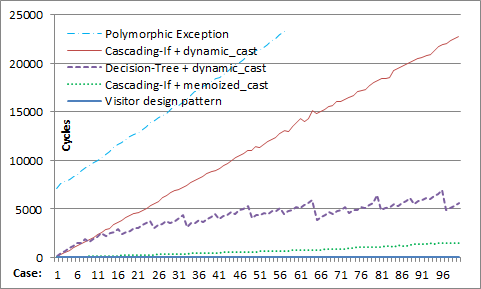
\includegraphics[width=0.47\textwidth]{DCast-vs-Visitors1.png}
  \caption{Type switching based on naive techniques}
  \label{fig:DCastVis1}
\end{figure}

When the class hiearchy is not flat and has several levels, the above 
cascading-if can be replaced with a decision tree that tests base classes first 
and thus eliminates many of the derived classes from consideration. This 
approach is used by Emir to deal with type patterns in Scala
\cite[\textsection 4.2]{EmirThesis}. The intent is to replace a sequence of 
independent dynamic casts between classes that are far from each other in the 
hierarchy with nested dynamic casts between classes that are close to each 
other. Another advantage is possiblity to fail early: if the type of the subject 
does not match any of the clauses, we will not have to try all the cases. 
Flat hierarchy, which will likely be formed by the leafs in even a multi-level 
hiearrchy, will not be able to benefit from this optimization and 
will effectively degrade to the above cascading-if. Nevertheless, when 
applicable, the optimization can be very useful and its benefits can be seen in
Figure~\ref{fig:DCastVis1} under ``Decision-Tree + dynamic\_cast''. The class 
hierarchy for this timing experiment was forming a perfect binary tree with 
classes number 2*N and 2*N+1 derived from a class with number N. The structure 
of the hierarchy also explains the repetitive pattern of timings.

The above solution either in a form of cascading-if or a decision tree can be 
significantly improved by lowering the cost of a single \code{dynamic_cast}. 
We devise an asymptotically constant version of this operator that we call
\code{memoized_cast} in \textsection\ref{sec:memcast}. As can be seen from the graph 
titled ``Cascading-If + memoized\_cast'', it speeds up the above cascading-if 
solution by a factor of 18 on average, as well as outperforms the decision-tree 
based solution for a number of case clauses way beyond those that can happen in 
a reasonable program. We leave the discussion of the technique until 
\textsection\ref{sec:memcast}, while we keep it in the chart to give perspective on 
an even faster solution to dynamic casting. The slowest implementation in the 
chart based on exception handling facilities of C++ is discussed in 
\textsection\ref{sec:xpm}.

The approach of Gibbs and Stroustrup employs divisibility of numbers to obtain a 
tag allocation scheme capable of performing type testing in constant time. 
Extended with a mechanism for storing offsets required for this-pointer 
adjustments, the technique can be used for an extremely fast dynamic casting on 
quite large class hierarchies\cite{FastDynCast}. The idea is to allocate tags 
for each class in such a way that tag of a class D is divisible by a tag of a 
class B if and only if class D is derived from class B. For comparison purposes 
we hand crafted this technique on the above flat and binary-tree hierarchies and 
then redid the timing experiments from Figure~\ref{fig:DCastVis1} using the fast 
dynamic cast. The results are presented in Figure~\ref{fig:DCastVis2}. For 
reference purposes we retained ``Visitor Design Pattern'' and ``Cascading-If + 
memoized\_cast'' timings from Figure~\ref{fig:DCastVis1} unchanged. Note that 
the Y-axis has been scaled-up 140 times, which is why the slope of 
``Cascading-If + memoized\_cast'' timings is so much bigger.

\begin{figure}[htbp]
  \centering
    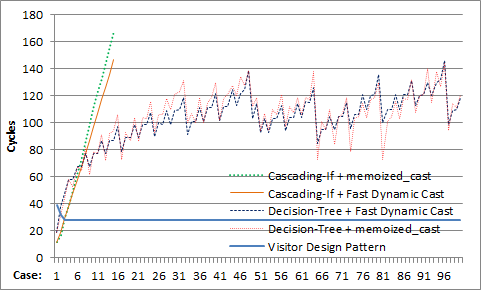
\includegraphics[width=0.47\textwidth]{DCast-vs-Visitors2.png}
  \caption{Type switching based on fast dynamic cast of Gibbs and Stroustrup\cite{FastDynCast}}
  \label{fig:DCastVis2}
\end{figure}

As can be seen from the figure the use of our memoized\_cast implementation can 
get really close in terms of performance to the fast dynamic cast, especially 
when combined with decision trees. An important difference that cannot be seen 
from the chart, however, is that the performance of memoized\_cast is 
asymptotic, while the performance of fast dynamic cast is guaranteed. This 
happens because the implementation of memoized\_cast will incure an overhead of 
a regular dynamic\_cast call on every first call with a given most derived type. 
Once that class is memoized, the performance will remain as shown. Averaged over 
all calls with a given type we can only claim we are asymptotically as good as 
fast dynamic cast.

Unfortunately fast dynamic casting is not truly open to fully satisfy our 
checklist. The structure of tags required by the scheme limits the amount of 
classes it can handle. A 32-bit integer is estimated to be able to represent 7 
levels of a class hierarchy that forms a binary tree (255 classes), 6 levels of 
a similar ternary tree hierarchy (1093 classes) or just one level of a hierarchy 
with 9 base classes -- multiple inheritance is the worst case scenario of the 
scheme that quickly drains its allocation possibilities. Besdies, similarly to 
other tag allocation schemes, presence of class extensions in DLLs will likely 
require an integration effort to make sure different DLLs are not reusing prime 
numbers in a way that might result in an incorrect dynamic cast.

Seeing predictably constant dispatching overhead of the visitor design pattern 
it became clear that any open solution that will have a non-constant dispatching 
overhead will have a poor chance of being adopted. Multi-way switch on 
sequentially allocated tags\cite{Spuler94} was one of the few techniques that 
could achieve constant overhead, and thus compete and even outperform visitors. 
Unfortunately the scheme has problems of its own that make it unsuitable.

%To better understand the problem let us look at some existing solutions to type 
%switching that we found to be used in practice. 

%From our experience on this project we have noticed that we can only compete 
%with visitors when switch statements are implemented with a jump table. As soon 
%as compiler was putting even a single branch into the decision tree of cases, 
%the performance was degraded significantly. From this perspective we do not 
%regard solutions based on decision trees as efficient, since they do not let us 
%compete compete with the visitors solution.

The simple scheme of assigning a unique tag per variant (instantiatable class 
here) will not pass our first question because the tags of base and derived 
classes will have to be different if the base class can be instantiated on its 
own. In other words we will not be able to land on a case label of a base class 
having a derived tag only. The already mentioned partitioning of tags of derived 
classes based on the classes in case clauses also will not help as it assumes 
knowledge of all the classes and thus fails extensibility through DLLs.

In practical implementations hand crafted for a specific class hierarchy, tags 
often are not chosen arbitrarily, but to reflect the subtyping relation of the 
underlain hierarchy. Switching on base classes in such setting will typically 
involve a call to some function $f$ that converts derived class' tag into a base 
class' tag. An example of such scheme would be having a certain bit in the tag 
set for all the classes derived from a given base class. Unfortunately this 
solution creates more problems then it solves.

First of all the solution will not be able to recognize an exceptional case 
where most of the derived classes should be handled as base class, while few 
should be handled specifically. Applying function $f$ puts several different 
types into an equivalence class with their base type, making them 
indistinguishable from each other.

Secondly, the assumed structure of tags is likely to make the set of tags 
sparce, effectively forcing compiler to use a decision tree instead of jump 
table to implement the switch. Even though conditional jump is reported to be 
faster than indirect jump on many computer architectures~\cite[\textsection 
4]{garrigue-98}, this did not seem to be the case in our experiments. Spliting 
of a jump table into two with a condition, that was sometimes happening because 
of our case label allocation scheme, was resulting in a noticable degradation of 
performance in comparison to a single jump table.

Besides, as was seen on the scheme of Gibbs and Stroustrup, the assumed 
structure of tags can also significantly decrease the amount of classes a given 
allocation scheme can handle. It is also interesting to note that even though 
their scheme can be easily adopted for type switching with decision trees, it is 
not easily adoptable for type switching with jump tables: in order to obtain 
tags of base classes we will have to decompose the derived tag into primes and 
then find all the dividers of the tag, present in case clauses.

Summarizing, truly open and efficient type switching seems to be a non trivial 
problem. The implementations we found in the literature where either open or 
efficient, but not both. Efficient implementation was typically achieved by 
sealing class hiearchy and using jump table. Without sealing, the implementation 
was resorting to decision trees and type testing, which was not efficient.
We are unaware of any efficient tag allocation scheme that can be used in a 
truly open scenario.

\section{Syntax and Semantics of our SELL} %%%%%%%%%%%%%%%%%%%%%%%%%%%%%%%%%%%%%
\label{sec:ss}

\subsection{Type Switch Syntax}
\label{sec:syn}

We present rather informally abstract syntax enabled by our SELL in order to 
improve clarity of the presentation. We do not try to capture all of the C++ 
syntax here because we do not in fact change or extend the language. All the 
facilities available through our library are nothing else but a syntactic sugar 
enabled through the ``clever'' use of template and macro mechanisms already 
present in the language. We do make use of several non-terminals from the C++ 
grammar to put the use of our constructs into context. For the complete C++ 
grammar we refer the curious reader to Appendix A of the current C++ 
standard\cite{C++0x}.

% TODO:
%()     Function call
%[]     Array subscripting
%*      Indirection (dereference)
%&      Address-of
%sizeof Size-of

\begin{center}
\begin{tabular}{rp{0em}cl}
\Rule{match statement}     & $M$       & \is{}  & \code{Match(}$e$\code{)} $\left[C s^*\right]^*$ \code{EndMatch} \\
\Rule{case clause}         & $C$       & \is{}  & \code{Case(}$\tau\left[,x\right]^*$\code{)} \\
                           &           & \Alt{} & \code{Otherwise(}$\left[,x\right]^*$\code{)} \\
\Rule{type-id}             & $\tau$    &        & C++\cite[\textsection A.7]{C++0x} \\
\Rule{statement}           & $s$       &        & C++\cite[\textsection A.5]{C++0x} \\
\Rule{expression}          & $e^\tau$  &        & C++\cite[\textsection A.4]{C++0x} \\
\Rule{identifier}          & $x^\tau$  &        & C++\cite[\textsection A.2]{C++0x} \\
\end{tabular}
\end{center}

\noindent                           
{\bf Match statement} is an analog of a switch statement that allows case 
clauses to be used as its case statements. We require it to be terminated with a 
dedicated \code{EndMatch} macro, to properly close the syntactic structure 
introduced with \code{Match} and followed by \code{Case},\code{Que} and 
\code{Otherwise} macros. Match statement will accept selectors of pointer and 
reference types, treating them uniformly in case clauses. This means that user 
does not have to mention \code{*,&} or any of the \code{const,volatile}-qualifiers
when specifying target types. Passing \code{nullptr} as a selector is considered 
\emph{ill-formed} however -- a choice we have made for performance reasons. 
Examples of match statement has already been presented in 
\textsection\ref{sec:intro} and \textsection\ref{sec:xmpl}.

We support three kinds of {\bf case clauses}: \code{Case}-\emph{clause}, 
\code{Que}-\emph{clause} and \code{Otherwise}-\emph{clause} also called 
\emph{default clause}. \code{Case} and \code{Que} clauses are refutable and both 
take a target expression as their first argument. \code{Otherwise} clause is 
irrefutable and can occur at most once among the clauses. Its target type is 
the selector type. \code{Case} and \code{Otherwise} clauses take additionally a 
list of identifiers that will be treated as variable patterns implicitly 
introduced into the clause's scope and bound to corresponding members of their 
target type. \code{Que} clause permits nested patterns as its arguments, but 
naturally requires all the variables used in the patterns to be explicitly 
pre-declared. Even though our default clause is not required to be the last 
clause of the match statement, we strongly encourage the user to place it 
last (hence the choice of name -- otherwise). Placing it at the beginning or in 
the middle of a match statement will only work as expected with \emph{tagged 
class} and \emph{discriminated union} encodings that use 
\emph{the-only-fit-or-default} strategy for choosing cases. The 
\emph{polymorphic base class} encoding uses \emph{first-fit} strategy and thus 
irrefutable default clause will effectively hide all subsequent case 
clauses, making them redundant. As we show in \textsection\ref{} the switch 
between \emph{polymorphic base class} and \emph{tagged class} encodings can 
simply be made with addition or removal a single definition, which may 
inadvertently change semantics of those match statements, where the default 
clause were not placed last.

When default clause takes optional variable patterns, it behaves in 
exactly the same way as \code{Case} clause whose target type is the selector 
type.

The remaining syntactic categories refer to non-terminals in the C++ grammar 
bearing the same name. {\bf Identifier} will only refer to variable names in our 
SELL, even though it has a broader meaning in the C++ grammar. {\bf Expression}
subsumes any valid C++ expression. We use expression $e^\tau$ to refer to a C++ 
expression, whose result type is $\tau$. {\bf Constant-expression} is a subset 
of the above restricted to only expression computable at compile time. {\bf 
Statement} refers to any valid statement allowed by the C++ grammar. Our match 
statement $M$ would have been extending this grammar rule with an extra case 
should it have been defined in the grammar directly. {\bf Type-id} represents a 
type expression that designates any valid C++ type. We are using this 
meta-variable in the superscript to other meta-variables in order to indicate a 
C++ type of the entity they represent.

\subsection{Semantics}
\label{sec:sem}

We use natural semantics\cite{Kahn87} (big-step operational semantics) to 
describe our pattern-matching semantics. As with syntax, we do not formalize the 
semantics of the entire language, but concentrate only on presenting relevant 
parts of our extension. We assume the entire state of the program is modeled by 
an environment $\Gamma$, which we can query as $\Gamma(x)$ to get a value of a 
variable $x$. In addition to meta-variables we have seen already, metavariables 
$u,v$ and $b^{bool}$ range over values. We make a simplifying assumption that 
all values of user-defined types are represented via variables of reference 
types and there exist a non-throwing operation \DynCast{\tau}{v} that can test 
whether an object of a given type is an instance of another type, returning a 
proper reference to it or a dedicated value \nullptr{} that represents 
\code{nullptr}. Intuitively, the semantics of such references is that of 
pointers in C++, which are implicitly dereferenced. We describe our semantics 
with several rule sets that deal with different parts of our syntax.

\subsubsection{Semantics of Match Statement}
\label{sec:semms}

Our second rule set deals with semantics of a \emph{match statement}. The 
judgements are of the form $\Gamma\vdash s \evals u,\Gamma'$ on statements, 
including match statement, and are slightly extended for case clauses 
$\Gamma\vdash_v C \evals u,\Gamma'$ with value $v$ of a selector that is passed 
along from the match statement onto the clauses.

\begin{mathpar}
\inferrule[Match-True]
{\Gamma \vdash e \evalspp v,\Gamma_1 \\ v \neq \nullptr \\
 \Gamma_1    \vdash_v C_1    \evals false,\Gamma_2 \\
 \Gamma_2    \vdash_v C_2    \evals false,\Gamma_3 \\
 \cdots \\
 \Gamma_{i-1}\vdash_v C_{i-1}\evals false,\Gamma_i \\
 \Gamma_i    \vdash_v C_i    \evals true, \Gamma_{i+1} \\
 \Gamma_{i+1}\vdash \vec{s}_i \evalspp u,\Gamma'
}
{\Gamma\vdash Match(e) \left[C_i \vec{s}_i\right]^*_{i=1..n} EndMatch \evals u,\Gamma'$\textbackslash$\{x | x \not\in \Gamma_i\}}
\end{mathpar}

\begin{mathpar}
\inferrule[Match-False]
{\Gamma \vdash e \evalspp v,\Gamma_1 \\ v \neq \nullptr \\
 \Gamma_1    \vdash_v C_1    \evals false,\Gamma_2 \\
 \Gamma_2    \vdash_v C_2    \evals false,\Gamma_3 \\
 \cdots \\
 \Gamma_{n-1}\vdash_v C_{n-1}\evals false,\Gamma_n \\
 \Gamma_n    \vdash_v C_n    \evals false,\Gamma_{n+1}
}
{\Gamma\vdash Match(e) \left[C_i \vec{s}_i\right]^*_{i=1..n} EndMatch \evals false,\Gamma_{n+1}}
\end{mathpar}

\begin{mathpar}
\inferrule[Case-Type]
{\Delta_i^{\tau} : \tau \rightarrow \tau_i, i=1..k \\
 \Gamma[x_i^{\tau_i}\rightarrow\tau_i()]_{i=1..k} $match$\langle\tau\rangle(x_1,...,x_k)(v) \evals u,\Gamma' \\
 \Gamma'' = (u \neq \nullptr\ ?\ \Gamma'[$matched$^\tau\rightarrow u] : \Gamma'$\textbackslash$\{x_i | i=1..k\})}
{\Gamma \vdash_v Case(\tau,x_1,...,x_k) \evals u,\Gamma''}
\end{mathpar}

\begin{mathpar}
\inferrule[Otherwise]
{\Gamma \vdash Case(\tau,\vec{x})(v) \evals true,\Gamma'}
{\Gamma \vdash_{v^\tau} Otherwise(\vec{x}) \evals true,\Gamma'}
\end{mathpar}

Evaluation of a match statement begins with evaluation of selector expression, 
which is not allowed to result in \code{nullptr}. This value is passed along to 
each of the clauses. The clauses are evaluated in their lexical order until the
first one that is not rejected. Statements associated with it are evaluated to 
form the outcome of the match statement. The resulting environment makes sure 
that local variables introduced by case clauses are not available after the 
match statement (\RefTirName{Match-True}). When none of the clauses were 
accepted, which is only possible when default clause was not specified, the 
resulting environment might still be different from the initial environment 
because of variables bound in partial matches during evaluation of clauses 
(\RefTirName{Match-False}).

Similarly to rules for \code{Que}-clause, the three rules for \code{Case}-clause 
only differ between themselves on the form of the target expression. Evaluation 
of the \code{Case}-clause begins with lookup for each of its $k$ arguments 
following target expression, the type of the value returned in the position $i$. 
Environment is then extended with default-initialized variables of those types. 
In practice, the variables are of reference type bound to either temporary or 
reference returned by $\Delta_i^{\tau,l}(u)$ so that no unnecessary copying is 
happening. A matching expression on a tree pattern is then executed to determine 
the acceptance of \code{Case}-clause. In case of success, the resulting 
environment will be augmented with locally bound variables passed as arguments 
as well as variable \code{matched} described above. In case of failure, the 
resulting environment might again contain the side-effects of partial matching, 
but will not introduce new variables into the environment (\RefTirName{Case-Type}, 
\RefTirName{Case-Layout} and \RefTirName{Case-View}).

Evaluation of default clause cannot fail because there is no \code{dynamic_cast} 
involved neither for the selector nor for implicit local variables: for the 
former the target type is by definition the selector type, while for the latter 
the type is chosen to be the type of expected values (\RefTirName{Otherwise}).

\section{Implementation} %%%%%%%%%%%%%%%%%%%%%%%%%%%%%%%%%%%%%%%%%%%%%%%%%%%%%%%
\label{sec:impl}

\subsection{Case of Polymorphic Classes}
\label{sec:copc}

As mentioned, we approach type switching on polymorphic classes and tagged 
classes differently. In this subsection we outline the implementation of type 
switching on classes that have vtbl pointer in their instances.

\subsubsection{Memoization Device}
\label{sec:memdev}

Let's look at a slightly more general problem than type switching. Consider a 
generalization of switch statement that takes predicates on a selector as its 
clauses and executes the first statement $s_i$ whose predicate got enabled: 

\begin{lstlisting}
switch (x)
{
    case P1(x): s1;
    ...
    case Pn(x): sn;
}
\end{lstlisting}

\noindent
Assuming that predicates depend only on $x$ and nothing else, we can be sure that
the next time we come to such switch with the same value, the same predicate 
will become enabled first. Thus, we would like to avoid evaluating predicates and 
jump straight to the statement it guards. In a way we would like the switch to 
memoize which case becomes enabled for a given value of $x$. 

Inspired by Duff's Device\cite{Duff} we devised a construct that we call 
\emph{Memoization Device} that does just that:

\begin{lstlisting}
typedef decltype(x) T;
static std::unordered_map<T,int> jump_target_map;

switch (int& target = jump_target_map[x])
{
default: // entered when we haven't seen x yet
    if (P1(x)) 
    {
        target = 1; // same as jump_target_map[x] = 1;
case 1: s1;
    } else 
    if (P2(x)) 
    {
        target = 2; // maps x to jump target 2
case 2: s2;
    } else
 ...
    if (Pn(x)) 
    {
        target = N; // maps x to jump target N
case N: sN;
    } else
        target = N+1; // maps x to switch' exit
case N+1:
}
\end{lstlisting}

The static \code{jump_target_map} maps values to jump targets, and will be 
allocated upon first entry to the function. The map is initially empty and is 
updated from within the switch as we proceed through the interleaved 
cascading-if statement. Accordingly to the logic of STL's \code{unordered_map}, 
a key $x$ that is not yet in the map will result in allocation of a new entry 
with its associated data (of type int) default initialized to 0. Since there is 
no case label 0 in the switch, default case will be taken, which, in turn, will 
initiate sequential execution of the interleaved cascading-if statement.

The sequential execution of the cascading-if statement will keep checking 
predicates $P_j(x)$ until the first predicate $P_i(x)$ that returns true. By 
assigning $i$ to \code{target} we will effectively associate $i$ with $x$ since 
\code{target} is just a reference to \code{jump_target_map[x]}. This association 
will make sure that the next time we are called with the value $x$ we will jump 
directly to the label $i$. When none of the predicates returns true, we will 
record it by associating $x$ with $N+1$, so that the next time we can jump 
directly to the end of the switch on $x$. 

The above construct effectively gives the entire statement first-fit semantics. 
In order to evaluate all the statements, whose predicates are true, and thus 
give the construct all-fit semantics, we might want to be able to preserve the 
fall-through behavior of the switch. In this case we can still skip the initial 
predicates returning false and start from the first successful one. This can be 
easily achieved by removing all else statements and making if-statements 
independent as well as wrapping all assignments to \code{target} with condition, 
to make sure only the first successful predicate executes it:

\begin{lstlisting}
 ...
    if (Pi(x)) { 
        if (target == 0)
            target = i;
case i:
        si;
    }
\end{lstlisting}

Note that the protocol that has to be maintained by this structure does not 
depend on the actual value of case labels. The only property we rely on here is 
that they are all different and that there is a predefined default value, 
distinct from any of them. In fact, the default clause we used here can be 
replaced with case clause with the predefined value. From experience, however, 
we have noticed that keeping the default clause results in a faster code. A more 
important performance consideration is to keep the values close to each other. 
Not following this rule might result in compiler choosing decision trees over a 
jump table implementation, which will significantly degrade the performance.

The first-fit semantics is not an inherent property of memoization device. 
Assuming that conditions are either mutually exclusive or imply one another we 
can build a decision-tree based memoization device that will effectively have 
\emph{most specific} semantics -- an analog of best-fit semantics in predicate 
dispatching\cite{ErnstKC98}.

Imagine that predicates with numbers $2i$ and $2i+1$ are mutually exclusive and 
each imply the value of the predicate with number $i$ i.e. $\forall x \in Domain(P)$
\begin{eqnarray*}
P_{2i+1}(x)\rightarrow P_i(x) \wedge P_{2i}(x)\rightarrow P_i(x) \wedge \neg(P_{2i+1}(x) \wedge P_{2i}(x))
\end{eqnarray*}
\noindent
The following decision-tree based memoization device will execute the statement 
$s_i$ associated with the \emph{most specific} (i.e. the predicate that implies 
all other predicates true on $x$) predicate $P_i$ that evaluates to true or will 
skip the entire statement if none of the predicates is true on $x$.

\begin{lstlisting}
switch (int& target = jump_target_map[x])
{
default:
    if (P1(x)) {
        if (P2(x)) {
            if (P4(x)) { target = 4; case 4: s4; } else
            if (P5(x)) { target = 5; case 5: s5; } 
            target = 2; case 2: s2;
        } else
        if (P3(x)) {
            if (P6(x)) { target = 6; case 6: s6; } else
            if (P7(x)) { target = 7; case 7: s7; } 
            target = 3; case 3: s3;
        }
        target = 1; case 1: s1;
    } else {
        target = 0; case 0:   ;
    }
}
\end{lstlisting}

An example of predicates that satisfy this condition are class membership tests
where the truth of a predicate that tests membership in a derived class implies 
the truth of a predicate that tests membership in its base class. Our library 
solution prefers the simpler cascading-if approach only because the necessary 
structure of the code can be layed out directly with macros. A compiler solution 
will use the decision-tree approach whenever possible to lower the cost of the 
first match from linear in case's number to logarithmic as senn in Figure\ref{fig:DCastVis1}.

The main advantage of memoization device is that it does not impose any 
restriction on the type of a selector. It can easily support multiple scrutinee 
by turning $x$ into a tuple. One has to be careful, however, to make sure the 
predicates do not involve global state. Another advantage is that conditions and 
statements do not have to be repeated several times textually, which lets us 
turn the boilerplate code of maintaining memoization logic into macros.

The main disadvantage of such solution is of course the size of table that grows 
proportionally to the amount of different values coming through the function. We 
will see, however, that often times the values can be grouped into equivalence 
classes, such that values in the same class do not change the predicate. The map 
can then associate an equivalence class with target.

\subsubsection{Virtual Table Pointers}
\label{sec:vtp}

Before we discuss our solution we would like to talk about certain properties of 
the C++ run-time system that we rely on. Strictly speaking C++ standard does not 
require implementations to use any given technique, however interoperability 
requirements have forced compiler vendors to design a set of rules called 
Application Binary Interface (ABI)\cite{C++ABI}. Most of the C++ compilers today 
follow these rules, with notable exception of Microsoft Visual C++. We show that 
the technique presented here will work with any C++ compiler that follows the 
C++ ABI. We also verified experimentally that Microsoft Visual C++ maintains the 
properties we rely on and thus our techniques are applicable to its current 
implementations as well.

Besides traditional single inheritance on classes, C++ supports 
multiple-inheritance of two kinds: repeated and virtual. Under repeated 
inheritance given derived class may inherit certain base class in several ways. 
Objects of such class will have several subobjects of that base class. Under 
virtual inheritance there will only be one shared subobject, accessible through 
different inheritance paths.

\begin{figure}[tbp]
  \centering
    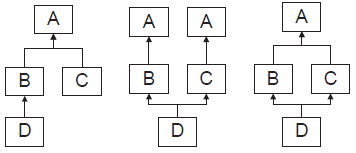
\includegraphics[width=0.47\textwidth]{Hierarchies.png}
  \caption{Single inheritance, repeated multiple inheritance and virtual multiple inheritance}
  \label{fig:hierarchy}
\end{figure}

\noindent
Note that the above picture portrais subobject relatedion, not the inheritance.

The notion of subobject has been formalized before\cite{RF95,WNST06,RDL11}.
We follow here the presentation of Ramamanandro et al\cite{RDL11}.

A base class subobject of a given complete object is represented by a pair 
$\sigma = \langle h,l\rangle$ with $h \in \{Repeated,Shared\}$ representing the 
kind of inheritance (single inheritance is repeated with one base class) and $l$ 
representing the path in non-virtual inheritance graph.

A predicate $C\leftY\sigma\rightY A$ they introduce means that $\sigma$ 
designates a base class subobject of class $C$, with subobject's static type 
being $A$. (Give recursive definition and more explanations from Layout paper).

A class that declares or inherits a virtual function is called a 
\emph{polymorphic class}\cite[\textsection 10.3]{C++0x}. C++ ABI in turn defines 
\emph{dynamic class} to be a class requiring a \emph{virtual table pointer} 
(because it or its bases have one or more virtual member functions or virtual 
base classes). A polymorphic class is thus a dynamic class by definition.

A \emph{primary base class} for a dynamic class is the unique base class (if any) 
with which it shares the virtual table pointer at offset 0. The data layout 
procedure for non-POD types described in \textsection2.4 of C++ ABI 
requires dynamic classes either to allocate vtable pointer at offset 0 or share 
the virtual table pointer from its primary base class, which is by definition at 
offset 0. For our purpose this means that we can rely on virtual table pointer 
always be present at offset 0 for dynamic classes.

C++ standard requires an argument of \code{dynamic_cast} to be a pointer to or 
an lvalue of a polymorphic type when performing \emph{downcast} -- a cast from 
base to derived.\cite[\textsection 5.2.7-6]{C++0x}. And since polymorphic type 
is dynamic type and dynamic types always have virtual table pointer at offset 0, 
we can safely extract such a pointer from an expression that was intended to be 
an argument of a \code{dynamic_cast} (e.g. from a type switch).

A dynamic class, accordingly to ABI, has an associated table (often several 
instances, but not one per object) called virtual table (or vtable). 
\emph{Virtual table} is a table of information used to dispatch virtual 
functions, access virtual base class subobjects, and to access information for 
runtime type identification (RTTI). \emph{Virtual table pointer} is a member of 
object's layout pointing to a virtual table. Because of repeated inheritance an 
object of given type may have several virtual table pointers in it. Each such 
pointer corresponds to one of the polymorphic base classes. 

Similarly, each class that has virtual member functions or virtual bases has an 
associated set of virtual tables. There may be multiple virtual tables for a 
particular class, if it is used as a base class for other classes. However, the 
virtual table pointers within all the objects (instances) of a particular 
most-derived class point to the same set of virtual tables.

The exact content of the virtual table is not important for this discussion. We 
would like to point out a few fields in it that we will refer to later.

\begin{itemize}
\item The \emph{typeinfo pointer} points to the typeinfo object used for RTTI. 
      It is always present.  
\item The \emph{offset to top} holds the displacement to the top of the object 
      from the location within the object of the virtual table pointer that 
      addresses this virtual table, as a \code{ptrdiff_t}. It is always present.
\item \emph{Virtual Base (vbase) offsets} are used to access the virtual bases 
      of an object. Such an entry is added to the derived class object address 
      (i.e. the address of its virtual table pointer) to get the address of a 
      virtual base class subobject. Such an entry is required for each virtual 
      base class.
\end{itemize}

\noindent
Given a virtual table pointer \code{vtbl}, we will refer to these fields as 
\code{rtti(vtbl)}, \code{off2top(vtbl)} and \code{vbase(vtbl)} respectively. 
Given an object $a$ of static type $A$ that has $k$ virtual table pointers in 
it, we will use the same notion we use for regular fields to access them: 
$a.vtbl_i$. We also assume presence of function $offset(\sigma)$ that defines 
the offset of the base class identified by the end of the path $\sigma$ within a 
class identified by its first element.

We would like to point out that during construction and deconstruction of an 
object, a value of a given virtual table pointer may change. In particular that 
value will reflect the dynamic type of the object to be the type of the fully 
constructed part only. This will not affect our reasoning, howver, as during 
such transition we treat the object to be the type of its fully constructed 
base only. Once the complete object is fully constructed, the value of the 
virtual table pointer will remain the same for the lifetime of the object.

\begin{theorem}
In an object layout that adheres to C++ ABI, virtual table pointers of two 
objects of the same static type are equivalent if and only if they have the same 
inheritance path in the same most-derived type.
%belong to the same subobject of 
\begin{eqnarray*}
    \forall a_1, a_2 : A\ |\ a_1\in C_1\leftY\sigma_1\rightY A \wedge a_2\in C_2\leftY\sigma_2\rightY A \\
    a_1.vtbl_i = a_2.vtbl_i \iff C_1 = C_2 \wedge \sigma_1 = \sigma_2
\end{eqnarray*}
\label{thm:vtbl}
\end{theorem}
\begin{proof}
Let's assume first $a_1.vtbl_i = a_2.vtbl_i$ but $C_1 \neq C_2$. In this case we 
have \code{rtti}$(a_1.vtbl_i) = $\code{rtti}$(a_2.vtbl_i)$. By definition 
\code{rtti}$(a_1.vtbl_i) = C_1$ while \code{rtti}$(a_2.vtbl_i) = C_2$, which 
contradicts that $C_1 \neq C_2$. Thus $C_1 = C_2 = C$.

Let's assume now that $a_1.vtbl_i = a_2.vtbl_i$ but $\sigma_1 \neq \sigma_2$. 
Let $\sigma_i=\langle h_i,l_i\rangle,i=1,2$ 

If $h_1 \neq h_2$ then one of them refers to virtual base while the other to 
repeated. Assuming $h_1$ refers to virtual path, \code{vbase}$(a_1.vtbl_i)$ has 
to be defined inside the vtable accordingly to ABI, while 
\code{vbase}$(a_2.vtbl_i)$ -- should not. This would contradict again that both 
$vtbl_i$ refer the same virtual table.

We have thus $h_1 = h_2 = h$. If $h = Shared$ than there is only one path to 
such $A$ in $C$, which would contradict $\sigma_1 \neq \sigma_2$. 
If $h = Repeated$ then we must have that $l_1 \neq l_2$. In this case let $k$ be 
the first position in which they differ: 
$l_1^j=l_2^j \forall j<k \wedge l_1^k\neq l_2^k$. Since our class $A$ is a base 
class for classes $l_1^k$ and $l_2^k$, both of which are in turn base classes of 
$C$, object identity requirement of C++ require that the relevant subobjects of 
type $A$ have different offsets within class $C$: 
$offset(\sigma_1)\neq offset(\sigma_2)$ However 
$offset(\sigma_1)=$\code{off2top}$(a_1.vtbl_i)=$\code{off2top}$(a_2.vtbl_i)=offset(\sigma_2)$ 
since $a_1.vtbl_i = a_2.vtbl_i$, which contradicts that offsets are different.

Conjecture in the other direction is trivial since subobjects on the same 
inheritance path in different instances will get initialized with the same 
vtable pointers.
\end{proof}

\begin{corollary}
Results of \code{dynamic_cast} can be reapplied to a different instance from within the same subobject.
$\forall a_1, a_2 : A\ |\ a_1.vtbl_i = a_2.vtbl_i \Rightarrow$
\code{dynamic_cast<B>}$(a_1).vtbl_j = $\code{dynamic_cast<B>}$(a_2).vtbl_j \vee$ \\
\code{dynamic_cast<B>}$(a_1)$ throws $\wedge$ \code{dynamic_cast<B>}$(a_2)$ 
throws.
\label{crl:vtbl}
\end{corollary}

\subsubsection{VTable Memoization}
\label{sec:vtblmem}

Since the results of dynamic cast can be reapplied on objects with the same 
virtual table pointer, we can now apply memoization device to polymorphic 
objects grouped by their virtual table pointer. The head of the switch requires 
few extra definitions:

\begin{lstlisting}
typedef std::pair<ptrdiff_t,size_t> type_switch_info;
static std::unordered_map<intptr_t, type_switch_info> jump_target_map;
intptr_t          vtbl = *reinterpret_cast<const intptr_t*>(p);
type_switch_info& info = jump_target_map[vtbl];
const void*       tptr; 
\end{lstlisting}

We use the virtual table pointer extracted from a polymorphic object pointed to 
by \code{p} as a key for association. The value stored along the key in 
association now keeps both: the target for the switch as well as a memoized 
offset for dynamic cast. The snippet corresponding to the $i^{th}$ case now 
looks as following:

\begin{lstlisting}
    if (tptr = dynamic_cast<const Di*>(p))
    {
        if (info.second == 0)
        {
            info.first  = intptr_t(tptr)-intptr_t(p);
            info.second = 42;
        }
case 42:
        auto matched = adjust_ptr<Di>(p,info.first); 
        si;
    }
\end{lstlisting}

\noindent
The main condition remains the same. We keep check for the first initialization 
because we allow the fall-through semantics here, letting user break from the 
switch when needed. Upon first entry we compute the offset that the dynamic cast 
performed and save it together with targed associated to the virtual table 
pointer. On the next iteration we will jump directly to the case label and 
restore the invariant of \code{matched} being a properly casted reference to the 
derived object.

\begin{figure}[htbp]
  \centering
    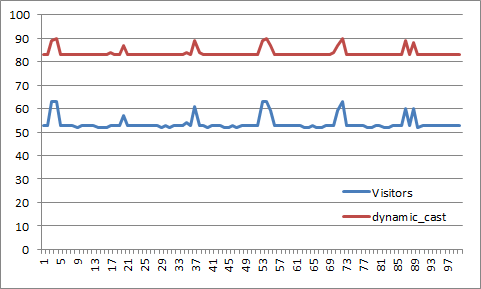
\includegraphics[width=0.47\textwidth]{DCast-vs-Visitors3.png}
  \caption{Time to uncover i\textsuperscript{th} case. X-axis - case i; Y-axis - cycles per iteration}
  \label{fig:DCastVis3}
\end{figure}

The net effect of this optimization can be seen in Figure~\ref{fig:DCastVis3}. 
We can see that the time does not increase with the position of the case we are 
handling. The spikes represent activities on computer during measurement and are 
present in both measurements. The type switch is still about 50\% slower, and 
making it even faster is discussed in the next subsection.

Note that we can apply the reasoning of \textsection\ref{sec:memdev} and change 
the first-fit semantics of the resulting match statement into a best-fit 
semantics simply by changing the underlain cascading-if structure with decision 
tree.

\subsubsection{Structure of Virtual Table Pointers}
\label{sec:sovtp}

Virtual table pointers are not entirely random addresses in memory and have 
certain structure when we look at groups of those that are associated with 
classes related by inheritance. Let us first look at some vtbl pointers that 
were present in some of our tests. The 32-bit pointers are shown in binary form 
(lower bits on the right) and are sorted in ascending order:

\begin{verbatim}
00000001001111100000011001001000
00000001001111100000011001011100
00000001001111100000011001110000
 ...
00000001001111100000011111011000
00000001001111100000011111101100
\end{verbatim}

These pointers are not constant values and are not even guaranteed to be the 
same between different runs of the same application. Techniques like 
\emph{address space layout randomization} or simple rebasing of the entire 
module are likely to change these values. The relative distance between them is 
likely to remain the same though as long as they come from the same module.

Comparing all the vtbl pointers that are coming through a given match statement 
we can trace ar run time the set of bits in which they do and do not differ. 
For the above example it may look as \texttt{00000001001111100000X11XXXXXXX00} 
where positions marked with X represent bits that are different in some vtbl 
pointers.

When a DLL is loaded it may have its own copy of v-tables for classes also used 
in other modules as well as v-tables for classes it introduces. Comparing 
similarly all vtbl pointers coming only from this DLL we can get a different 
pattern \\ \texttt{01110011100000010111XXXXXXXXX000} and when compared over all 
the loaded modules the pattern will likely becomes something like 
\texttt{0XXX00X1X0XXXXXX0XXXXXXXXXXXXX00}.

The common bits on the right come from the virtual table size and alignment 
requirements and depending on compiler, configuration and class hierarchy could 
easily vary from 2 to 6 bits. Because the vtbl pointer under C++ ABI points into 
an array of function pointers, the alignment requirement of 4 bytes for those 
pointers on a 32-bit architecture is what makes at least the last 2 bits to be 0. 
For our purpose the exact amount of bits on the right is not important as we 
evaluate this amount at run time based on vtbl pointers seen so far. Here we only 
would like to point out that there will be some amount of common bits on the 
right.

Another observation we made during our experiments with vtbl pointers of various 
existing applications was that the values of the pointers where changing more 
frequently in the lower bits than in the higher ones. We believe that this was 
happening because programers tend to group multiple derived classes in the same 
translation unit so the compiler was emitting virtual tables for them close to 
each other as well. 

Note also that derived classes that do not introduce their own virtual functions 
are likely to have virtual tables of the same size as their base class. Even 
when they do add new virtual functions the size of their virtual tables can only 
increase in comparison to their base classes. This is why the difference between 
many consequitive vtbl pointers that came through a given match statement was 
usually constant or very slightly different.

The changes in higher bits were typically due to separate compilation and 
especially due to dynamically loaded modules. Overally they were not changing 
the general tendancy we saw: smaller bits were changing more frequently than 
larger ones with the exception of lowest common bits of course.

With these observations in mind we introduced a cache on top of the hash table 
holding information about jump targets and the necessary offsets. The cache was 
using lowest non-common bits of the vtbl pointer to locate the necessary hash 
table information without consulting the hash table itself. The important 
guarantee about the validity of the cached hash table references comes from the 
C++0x standard, which states that ``insert and emplace members shall not affect 
the validity of references to container elements''\cite[\textsection 
23.2.5(13)]{C++0x}. 

Depending on the amount of actual collisions that happen in the cache our vtbl 
memoization technique can come close and even outperform the visitor design 
pattern. The numbers are, of course, averaged over many runs as the first run on 
every most derived type will take time shown in Figure\ref{fig:DCastVis1}. We 
did however test our technique on real code and can confirm that it does perform 
well in the real-world use cases.

The information about jump targets and necessary offsets is just an example of 
information we might want to be able to associate with and access via vtbl 
pointers. Our implementation of \code{memoized_cast} for example effectively 
reuses this general datastructure with a different type of element values. 
We thus created a generic reusable class \code{vtblmap<T>} that maps vtbl 
pointers to elements of type T. We will refer to the combined cache and 
hash-table data structure extended with the logic for minimizing conflicts 
presented below as \emph{vtblmap} data structure.

\subsubsection{Minimization of Conflicts}
\label{sec:moc}

Throughout this section by \emph{collision} we will call a run-time condition in 
which the cache entry of an incoming vtbl pointer is occupied by another vtbl 
pointer. Collision requires vtblmap to fetch the data associated with the new 
vtbl pointer from a slower hash-table and, under certain conditions, reconfigure 
cache for better performance. By \emph{conflict} we will call a different 
run-time condition under which given cache configuration maps two or more vtbl 
pointers to the same cache location. Presence of conflict does not necessarily 
imply presence of collisions, but collisions can only happen when there is a 
conflict. In the rest of this section we devise a mechanism that tries to 
minimize the amount of conflicts in a hope that it will also decrease the amount 
of actual collisions.

The amount of cycles that the visitor design pattern requires to uncover a type 
does not let us put sophisticated cache indexing mechanisms into the critical 
path of execution. This is why we limit our indexing function to shifts and 
masking operations as well as choose the size of cache to be a power of 2.

From the bit patterns of section \textsection\ref{sec:sovtp} we can see that 
given $n$ vtbl pointers we can always find a cache size that will render no 
conflicts between the vtbl pointers. The necessary size of such cache, however, 
can be too big to justify the use of memory. This is why in our current 
implementation we always consider only 2 different cache sizes: $2^k$ and 
$2^{k+1}$ where $2^{k-1} \le n \leq 2^k$. This guarantees us that the cache size 
is never more than 4 times bigger than the minimum required cache size.

During our experiments we noticed that often times the change in the last bit 
happens only in very few vtbl pointers, which effectively cuts the available 
cache space in half. To overcome this problem we let the amount of bits we 
shift the vtbl pointer by vary further and compute it in such a way that 
minimizes the number of conflicts.

To avoid doing any computations in the critical path \code{vtblmap} only 
reconfigures the optimal shift and the size of the cache when an actual collision 
happens: i.e. when it needs to fetch the value from a slower underlain hash 
table. In order to avoid constant recomputations when conflicts are unavoidable, 
we add an additional restriction of only reconfiguring the optimal parameters if 
the amount of vtbl pointers in the \code{vtblmap} has increased since the last 
recomputation. Since the amount of vtbl pointers is of the order $O(N)$, where 
$N$ is the finite amount of different classes in the loaded program, the 
restriction assures us that reconfigurations will not happen infinitely often.

To minimize the amount of recomputations even further, our library communicates 
to the \code{vtblmap<T>} through its constructor the amount of case clauses in 
the underlain match statement. We use this number as an estimate of expected 
size of \code{vtblmap} and pre-allocate the cache accordingly to this estimated 
number. The cache is still allowed to grow based on the actual amount of vtbl 
pointers that comes through a \code{vtblmap}, but it never shrinks from the 
initial value. This improvement significantly minimizes the amount of collisions 
at early stages as well as the number of possibilities we have to consider 
during reconfiguration.

The above logic of \code{vtblmap} always chooses the configuration that renders 
no conflicts, when such a configuration is possible during recomputation of 
optimal parameters. When this is not possible it is natural to prefer collisions 
to happen on less frequent vtbl pointers.

We studied frequency of vtbl pointers that come through various match statements 
on a C++ pretty-printer that we implemented on top of the Pivot 
framework\cite{Pivot09} using our pattern-matching library. We ran the pretty 
printer through a set of C++ standard library headers and then ranked all the 
classes from the most frequent to the least frequent ones on average. The 
resulting probability distribution is shown with a thicker line in 
Figure\ref{fig:PowerLaw}.

\begin{figure}[htbp]
  \centering
    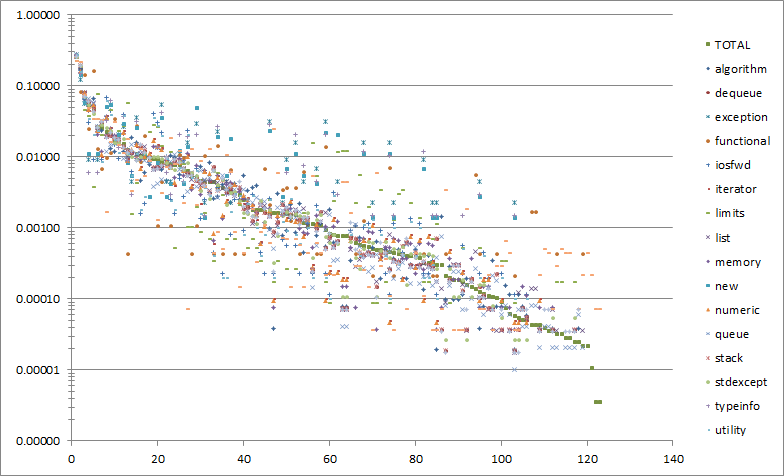
\includegraphics[width=0.47\textwidth]{std-lib-power-law-distributions.png}
  \caption{Probability distribution of various nodes in Pivot framework}
  \label{fig:PowerLaw}
\end{figure}

Note that Y-Axis is using logarithmic scale, suggesting that the resulting 
probability has power-law distribution. This is likely to be a specifics of our 
application, nevertheless, the above picture demonstrates that frequency of certain 
classes can be larger than the overall frequency of all the other classes. In 
our case the 2 most frequent classes were representing the use of a variable in 
a program, and their combined frequency was larger than the frequency of all the 
other nodes. Naturally we would like to avoid conflicts on such classes in the 
cache when possible.

Let us assume that a given \code{vtblmap} contains a set of vtbl pointers 
$V = \{v_1, ... , v_n\}$ with known probabilities $p_i$ of occuring. For a cache 
of size $2^k$ and a shift by $l$ bits we get a cache-indexing function 
$f_{lk} : V \rightarrow [0..2^k-1]$ defined as $f_{lk}(v_i) = (v_i \gg l) \& (2^k-1)$.
To calculate the probability of conflict for a given $l$ and $k$ parameters, let 
us consider $j^{th}$ cache cell and a subset $V^j_{lk}=\{v \in V | f_{lk}(v)=j\}$. 
When the size of this subset $m=|V^j_{lk}|$ is greater than 1, we have a 
potential conflict as subsequent request for a vtbl pointer $v''$ might be 
different from the vtbl pointer $v'$ currenly stored in the cell $j$. Within the 
cell only the probability of not having a conflict is the probability of both 
values $v''$ and $v'$ be the same:
\begin{eqnarray*}
P(v''=v')=\sum\limits_{v_i \in V^j_{lk}}P(v''=v_i)P(v'=v_i)=\sum\limits_{v_i \in V^j_{lk}}P^2(v_i|V^j_{lk})=\\
=\sum\limits_{v_i \in V^j_{lk}}\frac{P^2(v_i)}{P^2(V^j_{lk})}=
\sum\limits_{v_i \in V^j_{lk}}\frac{p_i^2}{(\sum\limits_{v_{i'} \in V^j_{lk}}p_{i'})^2}=
\frac{\sum\limits_{v_i \in V^j_{lk}}p_i^2}{(\sum\limits_{v_{i} \in V^j_{lk}}p_{i})^2}
\end{eqnarray*}

The probability of having a conflict among the vtbl pointers of a given cell is 
thus one minus the above value:

\begin{eqnarray*}
P(v''\neq v')=1-\frac{\sum\limits_{v_i \in V^j_{lk}}p_i^2}{(\sum\limits_{v_{i} \in V^j_{lk}}p_{i})^2}
\end{eqnarray*}

To obtain probability of conflict given any vtbl pointer and not just the one 
from a given cell we need to sum up the above probabilities of conflict within a 
cell multiplied by the probability of vtbl pointer fall into that cell:

\begin{eqnarray*}
P_{lk}^{conflict}=\sum\limits_{j=0}^{2^k-1}P(V^j_{lk})(1-\frac{\sum\limits_{v_i \in V^j_{lk}}p_i^2}{(\sum\limits_{v_{i} \in V^j_{lk}}p_{i})^2})=\\
=\sum\limits_{j=0}^{2^k-1}(\sum\limits_{v_{i} \in V^j_{lk}}p_{i})(1-\frac{\sum\limits_{v_i \in V^j_{lk}}p_i^2}{(\sum\limits_{v_{i} \in V^j_{lk}}p_{i})^2})
\end{eqnarray*}

Our reconfiguration algorithm then iterates over possible values of $l$ and $k$ 
and chooses those that minimize the overal probability of conflict $P_{lk}^{conflict}$.
The only data still missing are the actual probabilities $p_i$ used by the above 
formula. They can be approximated in many different ways.

Besides probability distribution on all the tests, Figure~\ref{fig:PowerLaw} 
shows probabilities of a given node on each of the tests. The X-Axis in this 
case represents the ordering of all the nodes accordingly to their overall rank 
of all the tests combined. As can be seen from the picture, the shape of each 
specific test's distribution still mimics the overal probability distribution. 
With this in mind we can simply let the user assign probabilities to each of the 
classes in the hierarchy and use these values during reconfiguration. The 
practical problem we came accross with this solution was that we wanted these 
probabilities be inheritable as Pivot separates interface and implementation 
classes and we prefered the user to define them on interfaces rather than on 
implementation classes. The easiest way to do so wast to write a dedicated 
function that would return the probabilities using a match statement. 
Unfortunately such a function will introduce a lot of overhead as it will 
ideally only be used very few times (since we try to minimize the amount of 
reconfiguration) and thus not be using memoized jumps but rather slow 
cascading-if.

A simpler and likely more precise way of estimating $p_i$ would be to count 
frequencies of each vtbl pointers directly inside the \code{vtblmap}. This 
introduces an overhead of an increment into the critical path of execution, but 
accordingly to our tests was only degrading the overal performance by 1-2\%.
Instead, it was compensating with a smaller amount of conflicts and thus a 
potential gain of performance. We leave the choice of whether the library should 
count frequencies of each vtbl pointer to the user of the library as the 
concrete choice may be to advantage on some class hierarchies and to 
disadvantage on others.

Figure~\ref{fig:Collisions} compares the amount of collisions when frequency 
information is and is not used. The data was gathered from 312 tests on multiple 
match statements present in Pivot's C++ pretty printer when it was ran over 
standard library headers. In 122 of these test both schemes had 0 conflicts and 
these tests are thus not shown on the graph. The remaining tests where ranked by 
the amount of conflicts in the scheme that does not utilize frequency information.

\begin{figure}[htbp]
  \centering
    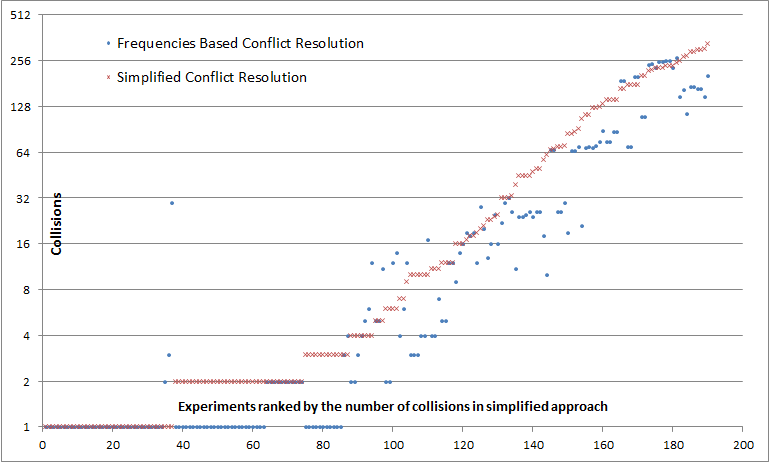
\includegraphics[width=0.47\textwidth]{CollisionsWithAndWithoutFrequencies.png}
  \caption{Decrease in number of collisions when probabilities of nodes are taken into account}
  \label{fig:Collisions}
\end{figure}

As can be seen from the graph, both schemes render quite low amount of 
collisions given that there was about 57000 calls in the rightmost test having 
the largest amount of conflicts. Taking into account that the Y-axis has 
logarithmic scale, the use of frequency information in many cases decreased the 
amount of conflicts by a factor of 2. The handfull of cases where the use of 
frequency increased the number of conflicts can be explained by the fact that 
the optimal values are not recomputed after each conflict, but after several 
conflicts and only if the amount of vtbl pointers in the vtblmap increased. These 
extra conditions sacrify optimality of parameters at any given time for the amount 
of times they are recomputed. By varying the number of conflicts we are willing 
to tolerate before reconfiguration we can decrease the number of conflicts by 
increasing the amount of recomputations and vise versa. From our experience, 
however, we saw that the drop in the number of conflicts was not translating 
into a proportional drop in execution time, while the amount of reconfigurations 
was proportional to the increase in execution time. This is why we choose to 
tolerate a relatively large amount of conflicts before recomputation just to 
keep the amount of recomputations low.

\subsection{Case of Tagged Classes}
\label{sec:cotc}

Memoization device outlined in \textsection\ref{sec:memdev} can in principle be 
applied to tagged classes too. The dynamic cast will be replaced by a small 
compile-time template meta-program that checks whether class associated with 
given tag is derived from the target type of the case clause. If so, the static 
cast can be used to obtain the offset.

Despite its straightforwardness we felt that it should be possible to do better 
than the general solution, given that each class is already identified with a 
dedicated constant known at compile time.

As we mentioned in \textsection\ref{sec:poets}, nominal subtyping of C++ 
effectively gives every class multiple types. The idea is thus to associate with 
the type not only its most derived tag, but also the tags of all its base classes.
In a compiler implementation such a list can be stored inside the vtable of a 
class, while in our library solution it is shared between all the instances with 
the same most derived tag in a less efficient global map, associating the tag to 
its tag list.

The list of tags is topologically sorted accordingly to the subtyping relation 
and terminates with a dedicated value distinct from all the tags. We call such a 
list a \emph{Tag Precedence List} (TPL) as it resembles the \emph{Class 
Precedence List} (CPL) of object-oriented descendants of Lisp (e.g. Dylan, 
Flavors, LOOPS, and CLOS) used there for \emph{linearization} of class 
hierarchies. The classes in CPL are ordered from most specific to least specific 
with siblings listed in the \emph{local precedence order} -- the order of the 
direct base classes used in the class definition. TPL is just an implementation 
detail and the only reason we distinguish TPL from CPL is that in C++ classes 
are often separated into interface and implementation classes and it might so 
happen that the same tag is associated by the user with an interface and several 
implementation classes. 

A type switch below, built on top of a hierarchy of tagged classes, proceeds as 
regular switch on the subject's tag. If the jump succeeds, we found an exact 
match, otherwise we get into a default clause that obtains the next tag in the 
tag precedence list and jump back to the beginning of the switch statement for a 
rematch:

\begin{lstlisting}
    const size_t* taglist = 0;
          size_t  attempt = 0;
          size_t  tag     = object->tag;
ReMatch:
    switch (tag) 
    {
    default:
        if (!taglist) 
            taglist = get_taglist(object->tag);
        tag = taglist[++attempt];
        goto ReMatch;
    case end_of_list: break;
    case bindings<D1>::kind_value: s1;
    ...
    case bindings<Dn>::kind_value: sN;
    }
\end{lstlisting}

The above structure lets us dispatch to case clauses of the most derived class 
with an overhead of initializing two local variables compared to a switch on a 
sealed hierarchy. Dispatching to a case clause of a base class will take a time 
roughly proportional to the distance between the matched base class and the most 
derived class in the inheritance graph. When none of the base class tags was 
matched we will necessarily reach the end\_of\_list marker in the tag precedence 
list and thus exit the loop.

Our library automatically builds the function \code{get_taglist} based on the 
\code{BC} or \code{BCS} specifiers that the user specifies in bindings 
(\textsection\ref{sec:bnd}).

To make the behavior clos

\begin{lstlisting}
    if (is_derived_from<Di>(object))
    {
case bindings<Di>::kind_value:
        auto matched = static_cast<Di>(object); 
        si;
    }
\end{lstlisting}


\subsection{(Ab)using Exceptions for Type Switching}
\label{sec:xpm}

Several authors had noted the relationship between exception handling and type 
switching before\cite{Glew99,ML2000}. Not surprisingly, the exception handling 
mechanism of C++ can be abused to implement the first-fit semantics of a type 
switch statement. The idea is to harness the fact that catch-handlers in C++ 
essentially use first-fit semantics to decide which one is going to handle a 
given exception. The only problem is to raise an exception with a static type 
equal to the dynamic type of selector.

To do this, we employ \emph{polymorphic exception} idiom\cite{PolyExcept} that 
introduces a virtual function \code{virtual void raise() const = 0;} into the 
base class, overriden by each derived class in syntactically same way: 
\code{throw *this;}. Match statement then simply calls \code{raise} on selector, 
while case clauses are turned into catch-handlers.
The exact name of the function is not important and can be communicated to the 
library as \emph{raise selector} with \code{RS} specifier in the same way 
\emph{kind selector} and \emph{class members} are (\textsection\ref{sec:bnd}). 
The \code{raise} member function can be seen as an analog of \code{accept} 
member function in visitor design pattern, whose main purpose is to discover 
subject's most specific type. The analog of call to \code{visit} to communicate 
that type is replaced in this scheme with exception unwinding mechanism.

Just because we can, it does not mean we should abuse the exception handling 
mechanism to give us the desired control flow. In the table-driven approach 
commonly used in high-performance implementations of exception handling, the 
speed of handling an exception is sacrificed to provide a zero execution-time 
overhead for when exceptions are not thrown\cite{Schilling98}. Using exception 
handling to implement pattern matching will reverse the common and exceptional 
cases, significantly degrading performance. As can be seen in 
Figure\ref{fig:DCastVis1}, matching the type of the first case clause with 
polymorphic exception approach takes more than 7000 cycles and then grows 
linearly (with the position of case clause in the match statement), making it the 
slowest approach. The numbers illustrate why exception handling should only be 
used to deal with exceptional and not common cases.

Despite its total inpracticality, the approach fits well into our unified syntax 
(\textsection\ref{sec:unisyn}) and gave us a very practical idea of harnessing a
C++ compiler to do \emph{redundancy checking} at compile time.

\subsubsection{Redundancy Checking}
\label{sec:redun}

As discussed in \textsection\ref{sec:bg}, redundancy checking is only applicable 
to first-fit semantics of the match statement, and warns the user of any 
case clause that will never be entered because of preceding one being more 
general.

We provide a library-configuration flag, which, when defined, effectively turns 
the entire match statement into a try-catch block with handlers accepting the 
target types of the case clauses. This forces the compiler to give warning when 
more general catch handler preceeds more specific one effectively performing a 
redundancy checking for us, e.g.:

\begin{lstlisting}
filename.cpp(55): warning C4286: 'ipr::Decl*' : is caught by 
                  base class ('ipr::Stmt*') on line 42
\end{lstlisting}

\noindent
Note that message contains both: a line number of the redundant case clause (55) 
and the line number of the case clause it is made redundant with (42).

Unfortunately the flag cannot be always enabled as case labels of the underlying 
switch statement have to be eliminated in order to render a syntactically 
correct program. Nevertheless, we found the redundancy checking facility of the 
library extremely useful when rewriting visitors based code: even though the 
order of overrides in visitor's implementation does not matter, for some reason 
more general ones were inclined to happen before specific ones in the code we 
looked at. Perhaps we are inclined to follow the class declaration order when 
defining and implementing visitors.

\subsection{Memoized Dynamic Cast}
\label{sec:memcast}

As seen from corollary~\ref{crl:vtbl} the results of \code{dynamic_cast} can be 
reapplied to a different instance from within the same subobject. This leads to 
a simple idea of memoizing the results of \code{dynamic_cast} and then using 
them on subsequent casts. In what follows we will only be dealing with the 
pointer version of the operator since the version on references that has a 
slight semantic difference can be easily implemented in terms of the pointer one.

The \code{dynamic_cast} operator in C++ involves two arguments: a value argument 
representing an object of a known static type as well as a type argument 
denoting the runtime type we are querying. It's behavior is twofold: on one side 
it should be able to determine when the object's most derived type is not a 
subtype of the queried type (or when the cast is ambiguous), while on the other 
it should be able to produce an offset to adjust the value argument by when it is.

We mimic the syntax of \code{dynamic_cast} by defining:

\begin{lstlisting}
template <typename T, typename S>
inline T memoized_cast(S* p);
\end{lstlisting}

\noindent
which lets the user replace all the uses of \code{dynamic_cast} in the program 
with \code{memoized_cast} with a simple:

\begin{lstlisting}
#define dynamic_cast memoized_cast
\end{lstlisting}

It is important to stress that the offset is not a function of source and target 
types of \code{dynamic_cast} operator, which is why we cannot simply memoize the 
outcome inside the individual instantiations of \code{memoized_cast}.
The use of repeated multiple inheritance will result in classes having several 
different offsets associated with the same pair of source and target types 
depending on which subobject the cast is performed from. Accordingly to 
corollary~\ref{crl:vtbl}, however, it is a function of target type and the value 
of the vtbl pointer stored in the object, because the vtbl pointer uniquely 
determines the subobject within the most derived type. Our memoization of 
results of \code{dynamic_cast} should thus be specific to a vtbl pointer and the 
target type. 

The easiest way to achieve this would be to use a dedicated global
\code{vtblmap<std::ptrdiff_t>} (\textsection\ref{sec:sovtp}) per each 
instantiation of the \code{memoized_cast}. This, however, will create an 
unnecessarily large amount of vtblmap structures, many of which will be  
duplicating information and repeating the work already done. This will happen 
because instantiations of \code{memoized_cast} with same target but different 
source types can share their vtblmap structures since vtbl pointers of different 
source types are necessarily different accordingly to Theorem~\ref{thm:vtbl}. 

Even though the above solution can be easily improved to allocates a single 
vtblmap per target type, an average application might have a lot of different 
target types. This is especially true for applications that will use our Match 
statement since we use \code{dynamic_cast} under the hood in each case clause. 
Indeed our C++ pretty printer was creating 160 vtblmaps of relatively small size 
each, which was increasing the executable size quite significantly because of 
numerous instantiations as well as noticably slowed down the compilation time.

To overcome the problem we turn each target type into a runtime instantiation 
index of the type and allocate a single \code{vtblmap<std::vector<std::ptrdiff_t>>} 
that associates vtbl pointers with a vector of offsets indexed by target type. 
The slight performance overhead that is brought by this improvement is specific 
to our library solution and would not be present in a compiler implementaion. 
Instead we get a much smaller memory footrpint, which can be made even smaller 
once we recognize the fact that global type indexing may effectively enumerate 
target classes that will never appear in the same Match statement. This will 
result in entries in the vector of offsets that are never used.

Our actual solution uses separate indexing of target types per each source type 
they are used with as well as allocates a different 
\code{vtblmap<std::vector<std::ptrdiff_t>>} for every source type. This lets us 
minimize unused entries within offset vectors by making sure only the plausible 
target types for a given source type are indexed. This solution should be 
suitable for most of the applications since we expect to have a fairly small 
amount of source types of \code{dynamic_cast} operator with a much larger amount 
of target types. For the unlikely case of small amount of target types and large 
amount of source types we let the user to revert the default behavior with a 
library confirugration switch that allocates a single vtblmap per target type as 
we have already discussed above.

Use of \code{memoized_cast} to implement match statement potentially reuses the 
results of \code{dynamic_cast} computation accross multiple independent match 
statements. This allows to leverage the cost of expensive first call with a 
given vtbl pointer even further accross all the match statements inside the 
program. The above define, with which a user can easily turn all dynamic casts 
into memoized casts can be used to speed-up existing code that uses dynamic 
casting without any refactoring overhead.

%\subsection{Discussion}
%\label{sec:dsc}

%Let us look at both our techniques in the context of Zenger and Odersky 
%challenge to independently extensible solutions of extension problem discussed 
%in \textsection\ref{sec:exp}.

%\begin{itemize}
%\item Extensibility in both dimensions: \\
%      %It should be possible to add new data variants, while adapting the 
%      %existing operations accordingly. It should also be possible to introduce 
%      %new functions. 
%      Our techniques allow one to extend data with subclassing as well as 
%      introduce new functions through a match statement on corresponding 
%      encoding. The existing operations 
%\item Strong static type safety: \\
%      %It should be impossible to apply a function to a data variant, which it 
%      %cannot handle.
%\item No modification or duplication: \\
%      %Existing code should neither be modified nor duplicated.
%\item Separate compilation: \\
%      %Neither datatype extensions nor addition of new functions should require 
%      %re-typechecking the original datatype or existing functions. No safety 
%      %checks should be deferred until link or runtime.
%\item Independent extensibility: \\
%      %It should be possible to combine independently developed extensions so 
%      %that they can be used jointly.
%\end{itemize}
%
\section{Evaluation} %%%%%%%%%%%%%%%%%%%%%%%%%%%%%%%%%%%%%%%%%%%%%%%%%%%%%%%%%%%
\label{sec:eval}

\begin{figure*}
\begin{tabular}{@{}c@{ }l||@{ }r@{}@{ }r@{}@{ }r@{}|@{ }r@{}@{ }r@{}@{ }r@{}||@{ }r@{}@{ }r@{}@{ }r@{}|@{ }r@{}@{ }r@{}@{ }r@{}||@{ }r@{}@{ }r@{}@{ }r@{}|@{ }r@{}@{ }r@{}@{ }r@{}}
\hline % -----------------------------------------------------------------------------------------------------------------------------------------
\hline % -----------------------------------------------------------------------------------------------------------------------------------------
 &            & \multicolumn{6}{c||}{G++/32}                  & \multicolumn{6}{c||}{MS Visual C++/32}        & \multicolumn{6}{c}{MS Visual C++/64}           \\
\hline % -----------------------------------------------------------------------------------------------------------------------------------------
 & Syntax     & \multicolumn{3}{c|}{Unified} & \multicolumn{3}{c||}{Specialized} & \multicolumn{3}{c|}{Unified} & \multicolumn{3}{c||}{Specialized} & \multicolumn{3}{c|}{Unified} & \multicolumn{3}{c}{Specialized} \\
\hline % -----------------------------------------------------------------------------------------------------------------------------------------
 & Encoding   & \Opn  & \Cls  & \Unn  & \Opn  & \Cls  & \Unn  & \Opn  & \Cls  & \Unn  & \Opn  & \Cls  & \Unn  & \Opn  & \Cls  & \Unn  & \Opn  & \Cls  & \Unn   \\
\hline % -----------------------------------------------------------------------------------------------------------------------------------------
\hline % -----------------------------------------------------------------------------------------------------------------------------------------
 & Repetitive &\gwNGPp&\gwNGKp&\gwNGUp&\gwNSPp&\gwNSKp&\gwNSUp&\vwNGPp&\vwNGKp&\vwNGUp&\vwNSPp&\vwNSKp&\vwNSUp&\vxNGPp&\vxNGKp&\vxNGUp&\vxNSPp&\vxNSKp&\vxNSUp \\
 & Sequential &\gwNGPq&\gwNGKq&\gwNGUq&\gwNSPq&\gwNSKq&\gwNSUq&\vwNGPq&\vwNGKq&\vwNGUq&\vwNSPq&\vwNSKq&\vwNSUq&\vxNGPq&\vxNGKq&\vxNGUq&\vxNSPq&\vxNSKq&\vxNSUq \\
 & Random     &\gwNGPn&\gwNGKn&\gwNGUn&\gwNSPn&\gwNSKn&\gwNSUn&\vwNGPn&\vwNGKn&\vwNGUn&\vwNSPn&\vwNSKn&\vwNSUn&\vxNGPn&\vxNGKn&\vxNGUn&\vxNSPn&\vxNSKn&\vxNSUn \\
\hline % ------------------------------------------------------------------------------------------------------------------------------------------
\multirow{3}{*}{\begin{sideways}{\tiny Forward}\end{sideways}}
 & Repetitive &\gwYGPp&\gwYGKp&\gwYGUp&\gwYSPp&\gwYSKp&\gwYSUp&\vwYGPp&\vwYGKp&\vwYGUp&\vwYSPp&\vwYSKp&\vwYSUp&\vxYGPp&\vxYGKp&\vxYGUp&\vxYSPp&\vxYSKp&\vxYSUp \\
 & Sequential &\gwYGPq&\gwYGKq&\gwYGUq&\gwYSPq&\gwYSKq&\gwYSUq&\vwYGPq&\vwYGKq&\vwYGUq&\vwYSPq&\vwYSKq&\vwYSUq&\vxYGPq&\vxYGKq&\vxYGUq&\vxYSPq&\vxYSKq&\vxYSUq \\
 & Random     &\gwYGPn&\gwYGKn&\gwYGUn&\gwYSPn&\gwYSKn&\gwYSUn&\vwYGPn&\vwYGKn&\vwYGUn&\vwYSPn&\vwYSKn&\vwYSUn&\vxYGPn&\vxYGKn&\vxYGUn&\vxYSPn&\vxYSKn&\vxYSUn \\
\hline % -----------------------------------------------------------------------------------------------------------------------------------------
\hline % -----------------------------------------------------------------------------------------------------------------------------------------
 &            & \multicolumn{6}{c||}{G++/32}                  & \multicolumn{6}{c||}{MS Visual C++/32 with PGO} & \multicolumn{6}{c}{MS Visual C++/64 with PGO} \\
\hline % -----------------------------------------------------------------------------------------------------------------------------------------
 & Syntax     & \multicolumn{3}{c|}{Unified} & \multicolumn{3}{c||}{Specialized} & \multicolumn{3}{c|}{Unified} & \multicolumn{3}{c||}{Specialized} & \multicolumn{3}{c|}{Unified} & \multicolumn{3}{c}{Specialized} \\
\hline % -----------------------------------------------------------------------------------------------------------------------------------------
 & Encoding   & \Opn  & \Cls  & \Unn  & \Opn  & \Cls  & \Unn  & \Opn  & \Cls  & \Unn  & \Opn  & \Cls  & \Unn  & \Opn  & \Cls  & \Unn  & \Opn  & \Cls  & \Unn   \\
\hline % -----------------------------------------------------------------------------------------------------------------------------------------
\hline % -----------------------------------------------------------------------------------------------------------------------------------------
 & Repetitive &\GwNGPp&\GwNGKp&\GwNGUp&\GwNSPp&\GwNSKp&\GwNSUp&\VwNGPp&\VwNGKp&\VwNGUp&\VwNSPp&\VwNSKp&\VwNSUp&\VxNGPp&\VxNGKp&\VxNGUp&\VxNSPp&\VxNSKp&\VxNSUp \\
 & Sequential &\GwNGPq&\GwNGKq&\GwNGUq&\GwNSPq&\GwNSKq&\GwNSUq&\VwNGPq&\VwNGKq&\VwNGUq&\VwNSPq&\VwNSKq&\VwNSUq&\VxNGPq&\VxNGKq&\VxNGUq&\VxNSPq&\VxNSKq&\VxNSUq \\
 & Random     &\GwNGPn&\GwNGKn&\GwNGUn&\GwNSPn&\GwNSKn&\GwNSUn&\VwNGPn&\VwNGKn&\VwNGUn&\VwNSPn&\VwNSKn&\VwNSUn&\VxNGPn&\VxNGKn&\VxNGUn&\VxNSPn&\VxNSKn&\VxNSUn \\
\hline % ------------------------------------------------------------------------------------------------------------------------------------------
\multirow{3}{*}{\begin{sideways}{\tiny Forward}\end{sideways}}
 & Repetitive &\GwYGPp&\GwYGKp&\GwYGUp&\GwYSPp&\GwYSKp&\GwYSUp&\VwYGPp&\VwYGKp&\VwYGUp&\VwYSPp&\VwYSKp&\VwYSUp&\VxYGPp&\VxYGKp&\VxYGUp&\VxYSPp&\VxYSKp&\VxYSUp \\
 & Sequential &\GwYGPq&\GwYGKq&\GwYGUq&\GwYSPq&\GwYSKq&\GwYSUq&\VwYGPq&\VwYGKq&\VwYGUq&\VwYSPq&\VwYSKq&\VwYSUq&\VxYGPq&\VxYGKq&\VxYGUq&\VxYSPq&\VxYSKq&\VxYSUq \\
 & Random     &\GwYGPn&\GwYGKn&\GwYGUn&\GwYSPn&\GwYSKn&\GwYSUn&\VwYGPn&\VwYGKn&\VwYGUn&\VwYSPn&\VwYSKn&\VwYSUn&\VxYGPn&\VxYGKn&\VxYGUn&\VxYSPn&\VxYSKn&\VxYSUn \\
\hline % -----------------------------------------------------------------------------------------------------------------------------------------
\end{tabular}
\caption{Relative performance of our pattern matching versus visitors. Numbers 
like \f{42} in bold font indicate that our pattern matching is faster than 
visitors by corresponding percentage. Numbers like \s{42} in italics font 
indicate that our solution is slower than visitors (i.e. visitors is faster than 
our solution) by corresponding percentage.}
\label{relperf}
\end{figure*}

In this section we evaluate the performance of our solution in comparison to its 
de facto contender -- visitor design pattern. We also compare performance of 
some typical uses cases expressed with our solution and OCaml.

Our evaluation methodology consists of several benchmarks that we believe 
represent various possible uses of objects analized with either visitors or 
pattern matching.

\emph{Repetitive} benchmark performs multiple calls on different objects of the 
same most derived type. This scenario happens in object-oriented setting when a 
group of polymorphic objects is created and passed around (e.g. numerous 
particles of a given kind in a particle simulation system). We include it 
because double dispatch becomes about twice faster (27 vs 53 cycles) in this 
scenario compared to others due to cache and call target prediction mechanisms. 

\emph{Sequential} benchmark effectively uses object of each derived type only 
once and then moves on to an object of a different type. The cache is typically 
reused the least in this scenario. The scenario is typical of lookup tables, 
where each entry is implemented with a different derived class.

\emph{Random} benchmark is the most representative as it randomly makes calls on 
random objects, which will probably be the most common usage scenario in the 
real world.

\emph{Forwarding} benchmark is not a benchmark on its own, but rather a 
combinator that can be applied to any of the above scenarios. It refers to the 
common technique used by visitors where for class hierarchies with multiple 
levels of inheritance the \code{visit} method of a derived class will provide a 
default implementation of forwarding to its immediate base class, who in turn 
may forward it to its base class etc. This approach is used in Pivot, whose AST 
hierarchy consists of 154 node kinds, of which only 5 must be handled, while the 
rest will forward to them when visit for them was not overriden.

These benchmarks were executed in the following configurations:

\begin{itemize}
\item Sony VAIO\textsuperscript{\textregistered} laptop with Intel\textsuperscript{\textregistered} Core\texttrademark i5 460M 
      Processor at 2.53 GHz equipped with 6GB of RAM running Windows 7 
      Professional
      \begin{itemize}
      \item G++ 4.5.2 under MinGW executed with -O2 and producing x86 binary
      \item MS Visual C++ 2010 Professional
            \begin{itemize}
            \item x86 binary
            \item x64 binary
            \item x86 binary with Profile Guided Optimizations
            \item x64 binary with Profile Guided Optimizations
            \end{itemize}
      \end{itemize}
\end{itemize}

Each benchmark under each configuration were tested with either \emph{unified} 
or \emph{specialized} syntax. Each syntax was used to run tests on \emph{Open} 
(generalization of \emph{polymorphic base class} encoding), \emph{Tag} 
(generalization of \emph{tag class} encoding) and \emph{Union} (same as 
\emph{discriminated union} encoding). Specialized syntax avoids generating 
unnecessary syntactic structure used to unify syntax and thus produces faster 
code. We include it in results as compiler implementation of pattern matching 
will be able to distinguish each case and thus generate only the required 
structure.

We include results of optimizing code created with Visual C++ by using profile 
guided optimizations as currently Visual C++ does not have means for branch 
hinting, which are supported by G++ and proven to be very effective in few 
cruicial places. Profile guided optimization in Visual C++ lets compiler find 
out experimentally what we would have otherwise hinted, even though this 
includes other optimizations as well.

We compare performance of our solution relatively to performance of visitors in 
Figure~\ref{relperf}. The values are given as percentage of performance increase 
against the slower technique. Numbers in bold represent cases where our pattern 
matching was faster than visitors and indicate corresponding percentage. Numbers 
in italics indicate cases where visitors were faster (and thus we were slower) 
by given percentage.

From the numbers given we can see that pattern matching wins by a good margin in 
the presense of at least one level of forwarding on visitors. Using pattern 
matching on closed hierarchies is a definite winner that providing the same 
unified syntax. Use of specialized syntax always results in a faster pattern 
matching code by avoiding unification overhead.

The code for x64 is only slower relatively: the actul time spent for both 
visitors and pattern matching was smaller than that for x86, but it was much 
smaller for visitors than pattern matching, which resulted in worse relative 
performance.

\section{Related Work} %%%%%%%%%%%%%%%%%%%%%%%%%%%%%%%%%%%%%%%%%%%%%%%%%%%%%%%%%
\label{sec:rw}

There are two main approaches to compiling pattern matching code: the first is 
based on \emph{backtracking automata} and was introduced by Augustsson\cite{}, 
the second is based on \emph{decision trees} and is attributed in the literature 
to Dave MacQueen and Gilles Kahn in their implementation of Hope compiler \cite{}.
Backtracking approach usually generates smaller code, while decision tree 
approach produces faster code by ensuring that each primitive test is only 
performed once. Neither of the approaches addresses specifically type patterns 
or type switching and simply assumes presence of a primitive operation capable 
of performing type tests.

Memoization device we proposed is not specifically concerned with compiling 
pattern matching and can be used independently. In particular it can be combined 
with either backtracking or decision tree approaches to avoid subsequent 
decisions on datum that has already been seen.

%xxxxxxxxxxxxxxxxxxxxxxxxxxxxxxxxxxxxxxxxxxxxxxxxxxxxxxxxxxxxxxxxxxxxxxx

\emph{Extensible Visitors with Default Cases}\cite[\textsection 
4.2]{Zenger:2001} attempt to solve the extensibility problem of visitors, 
however the solution, after 
remapping it onto C++, has problems of its own. The visitation interface 
hierarchy can easily be grown linearly (adding new cases for the new classes in 
the original hierarchy each time), but independent extensions by different  
authorities require developer's intervention to unify them all, before they can 
be used together. This may not be feasible in environments that use dynamic 
linking. To avoid writing even more boilerplate code in new visitors, the 
solution would require usage of virtual inheritance, which typically has 
an overhead of extra memory dereferencing. On top of the double dispatch already 
present in the visitor pattern, the solution will incur two additional virtual 
calls and a dynamic cast for each level of visitor extension. Additional double 
dispatch is incurred by forwarding of default handling from base visitor to a 
derived one, while the dynamic cast is required for safety and can be replaced 
with a static case when visitation interface is guaranteed to be grown linearly 
(extended by one authority only). Yet another virtual call is required to be 
able to forward computations to subcomponents on tree-like structures to the 
most derived visitor. This last function lets one avoid the necessity of using 
heap to allocate a temporary visitor through the \emph{Factory Design 
Pattern}\cite{DesignPatterns1993} used in \emph{Extensible Visitor} solution 
originally proposed by Krishnamurti, Felleisen and Friedman\cite{Krishnamurthi98}.

In order to address expression problem in Haskell, L\"{o}h and Hinze proposed to 
extend its type system with open data types and open functions\cite{LohHinze2006}.
Their solution allows the user to mark top-level data types and functions as 
open and then provide concrete variants and overloads anywhere in the program. 
The semantics of open extension is given by transformation into a single module, 
where all the definitions are seen in one place. While open data types introduce 
some of the problems that subclassing does in object-oriented languages, the 
problems are simpler. As we discussed before, the object-oriented analog of 
adding new variants is addition of a class that implements a given interface. In 
other words it is a derived class that extends a strictly flat class hierarchy. 
This largely avoids the problem of classes having multiple types and thus the 
problem of type switching on base classes. Another limitation of their approach 
that prevents from calling it a truly open solution is the fact that their 
semantics essentially assumes a whole program view, which excludes any 
extensions via DLLs. As is the case with many other implementations of open 
extensions authors rely on the closed world for efficient implementation: in 
their implementation \emph{data types can only be entirely abstract (not 
allowing pattern matching) or concrete with all constructors with the reason 
being that pattern matching can be compiled more efficiently if the layout of 
the data type is known completely}. The authors also believe that \emph{there 
are no theoretical difficulties in lifting this restriction, but it might imply 
a small performance loss if closed functions pattern match on open data types}. 
Our work addresses exactly this problem, showing that it is not only 
theoretically possible but also practically efficient and in application to a 
broader problem.

Polymorphic variants in OCaml\cite{garrigue-98} allow addition of new variants 
later. They are simpler, however, than object-oriented extensions as they do not 
form subtyping between variants themsevles, but only between combinations of them. 
This makes an impportant distinction between \emph{extensible sum types} like 
polymorphic variants and \emph{extensible hierarhical sum types} like classes.
An important property of extensible sum types is that each value of the 
underlain algebraic data type belongs to exactly one disjoint subset tagged with 
a constructor. The \emph{nominative subtyping} of object-oriented languages does 
not usually have this disjointness making classes effectively have multiple 
types. In particular, the case of disjoint constructors can be seen as a 
degenerated case of a flat class hierarchy among the multitude of possible class 
hierarchies.

Tom is a pattern matching compiler that can be used together with Java, C or 
Eiffel to bring a common pattern matching and term rewriting syntax into the 
languages\cite{Moreau:2003}. It works as a preprocessor that transforms 
syntactic extensions into imperative code in the target language. Tom is quite 
transparent as to the concrete target language used and can potentially be 
extended to other target languages besides the three supported now. In 
particular, it never uses any semantic information of the target language during 
the compilation process and it does not inspect nor modify the source language 
part (their preprocessor is only aware of parenthesis and block delimiters of 
the source language). Tom has a sublanguage called Gom that can be used to 
define algebraic data types in a uniform mannaer, which their preprocessor then 
transforms into conrete definitions in the target language. Alternatively, the 
user can provide mappings to his own data structures that the preprocessor will 
use to generate the code.

In comparison to our approach Tom has much bigger goals. The combination of 
pattern matching, term rewriting and strategies turns Tom into a 
tree-transformation language similar to Stratego/XT, XDuce and others. 
The main accent is made on expressivity and the speed of development, which 
makes one often wonder about the run-time complexity of the generated code.
Tom's approach is also prone to general problems of any preprocessor based 
solution\cite[\textsection 4.3]{SELL}. For example, when several preprocessors 
have to be used together, each independent extension may not be able to 
understand the other's syntax, making it impossible to form a toolchain.
A library approach we follow avoids most of these problems by relying only on a 
standard C++ compiler. It also lets us employ semantics of the language within 
patterns: e.g. our patterns work directly on underlying user-defined data 
structures, largely avoiding abstraction penalties. A tighter integration with 
the language semantics also makes our patterns first-class citizens that can be 
composed and passed to other functions. The approach we take to type switching 
can also be used by Tom's preprocessor to implement type patterns efficiently -- 
similarly to other object-oriented languages, Tom's handling of them is based on 
highly inefficient \code{instanceof} operator and its equivalents in other 
languages.

%An example would be our generalized n+k patterns where we 
%can turn any invertible function even user defined into a pattern.

There has been previous attempts to use pattern matching with the Pivot 
framework that we used to experiment with our library. In his dissertation, 
Pirkelbauer devised a pattern language capable of representing various entities 
in a C++ program. The patterns were then translated with a tool into a set of 
visitors implementing the underlain pattern matching 
semantics\cite{PirkelbauerThesis}. Earlier, Cook et al used expression templates 
to implement a query language for Pivot's Internal Program Representation 
\cite{iql04}. While their work was built around a concrete class hierarchy 
letting them put some semantic knowledge about concrete classes into the 
The principal difference of their work from this work is that 
authors were essentially creating a pattern matcher for a given class hierarchy 
and thus could take the semantics of the entities represented by classes in the 
hierarchy into account. Our approach is parametrized over class hierarchy and 
thus provides a rather lower level pattern-matching functionality that lets one 
simplify work with that hierarchy.  One can think of it as a generalized 
dynamic\_cast. To be continued...

\section{Future Work} %%%%%%%%%%%%%%%%%%%%%%%%%%%%%%%%%%%%%%%%%%%%%%%%%%%%%%%%%%
\label{sec:fw}

The current implementation of our library relies on static variables and global 
state. This will have problems in a multi-threaded environment so the first 
extension we would like to provide is an efficient multi-threaded 
implementation.

Match statement that we presented here deals with only one scrutiny at the 
moment, but we believe that memoization device along with vtable caching 
technique we presented can cope reasonably efficiently with multiple scrutinies. 
Their support will make our library more general by addressing asymmetric 
multiple dispatch.

Containers as described by the standard C++ library do not have the implicit 
recursive structure present in lists, sequences and other recursive data 
structures of functional languages. Viewing them as such with view will likely 
have a significant performance overhead, not usually affordable in the kind of 
applications C++ is used for. We therefore would like to experiment with some 
pattern matching alternatives that will let us work with STL containers 
efficiently yet expressively as in functional languages.

\section{Conclusions} %%%%%%%%%%%%%%%%%%%%%%%%%%%%%%%%%%%%%%%%%%%%%%%%%%%%%%%%%%
\label{sec:cc}

We described three techniques that can be used to implement type switching, type 
testing, pattern matching, predicate dispatching and other facilities that 
depend on a run-time type of an argument.

\emph{Memoization Device} is an optimization technique that maps run-time values 
to execution paths, allowing to take shortcuts on subsequent runs with the same 
value. The technique does not require code duplication and in typical cases adds 
only a single indirect assignment to each of the execution paths. It can be 
combined with other compiler optimizations and is particularly suitable for use 
in a library setting.

\emph{V-Table Memoization} is technique based on memoization device that employs 
certain properties of virtual table pointers to not only speed up execution, but 
also properly uncover dynamic type of an object. This technique is a backbone of 
our fast type switch as well as memoized dynamic cast optimization.

\emph{Tag Preceedence List} is yet another technique that can be used to 
implement best-fit type switching on tagged classes. The technique has its pros 
and cons in comparison to v-table memoization, which we discuss in the paper.

These techniques can be used in a compiler and library setting and support well 
separate compilation and dynamic linking. They are open to class extensions and 
interact well with other C++ facilities such as multiple inheritance (including 
repetitive and virtual inheritance) and templates. The techniques are not 
specific to C++ and can be adopted in other languages for similar purposes.

Using the above techniques we implemented a library for efficient type switching 
in C++. Our implementation comes close or outperforms its closest contender -- 
visitor design pattern as well as overcomes the restrictions, inconveniences and 
difficulties in teaching and using, typically associated with it.

We used the library to rewrite an existing code that was relying heavily on 
visitors and discovered that resulting code became much shorter, simpler, easier 
to maintain and comprehend.

\bibliographystyle{abbrvnat}
\bibliography{mlpatmat}
\end{document}
